\documentclass[a4paper]{iacas}

\usepackage{cite}
\usepackage{hyperref}% embedding hyperlinks [must be loaded after dropping]
\usepackage{amsmath,amsthm,amssymb,amsfonts,latexsym,mathrsfs,wasysym}
\usepackage{marvosym}
\usepackage{subcaption}
\usepackage{soul,color}
\usepackage{threeparttable}% tables with footnotes
\usepackage{dcolumn}% decimal-aligned tabular math columns
\usepackage{float}
\usepackage{graphicx}
\usepackage{accents}
\usepackage{tikz}
\usepackage{lastpage}
\usepackage{fancyhdr}
\usepackage{color}
\usepackage{cancel}
\usepackage{setspace}
%\doublespacing
% or:
\onehalfspacing
%\usepackage[T1]{fontenc}
%\usepackage{bigfoot} % to allow verbatim in footnote
\usepackage[framed,numbered]{matlab-prettifier}
\pagestyle{plain}
%\usepackage[hebrew,english]{babel}
\usetikzlibrary{shapes.geometric, arrows, calc}

\newcolumntype{d}{D{.}{.}{-1}}
\graphicspath{{figures/}}

% define some commands to maintain consistency
\newcommand{\pkg}[1]{\texttt{#1}}
\newcommand{\cls}[1]{\textsf{#1}}
\newcommand{\file}[1]{\texttt{#1}}
\newcommand{\sgn}[1]{\operatorname{sgn}\left(#1\right)}
\newcommand{\sat}[1]{\operatorname{sat}\left(#1\right)}
\newcommand{\rrule}[1]{\rule[#1]{0pt}{0pt}}
\newcommand{\fracds}[2]{\frac{\displaystyle #1\rrule{-0.2em}}{\displaystyle #2\rrule{1em}}}
\newcommand{\figref}[1]{Fig.~\ref{#1}}
\newcommand{\ubar}[1]{\underaccent{\bar}{#1}}
\newcommand{\norm}[1]{\lvert \lvert \vec #1 \rvert \rvert}

%diffeomorphism

\begin{document}

\begin{center}
 \large Algorithms and Application in Computer Vision - 046746
 \end{center}
\begin{center}
\large\textbf{Homework \#1}
 \end{center}


\begin{tabular}{l}
\\
{\bf\textit{Alexander Shender 328626114}} \\
{\bf\textit{Vladimir Tchuiev 309206795}} \\
Technion - Israel Institute of Technology
\end{tabular}

\vspace{2em}

\section{Part 2}

\subsection{Part 2a}

In this part we built a Laplacian of Gaussians (LoG) pyramid. Fig.~\ref{fig:LoG} presents the LoG pyramid for 4 levels of the building image, with each level progressively shows rougher edges, with 0 being black. The lower pyramid level, the more detail it shows, with the highest level being "background".

\begin{figure}[!htbp]
	
	\begin{subfigure}[b]{0.23\textwidth}
		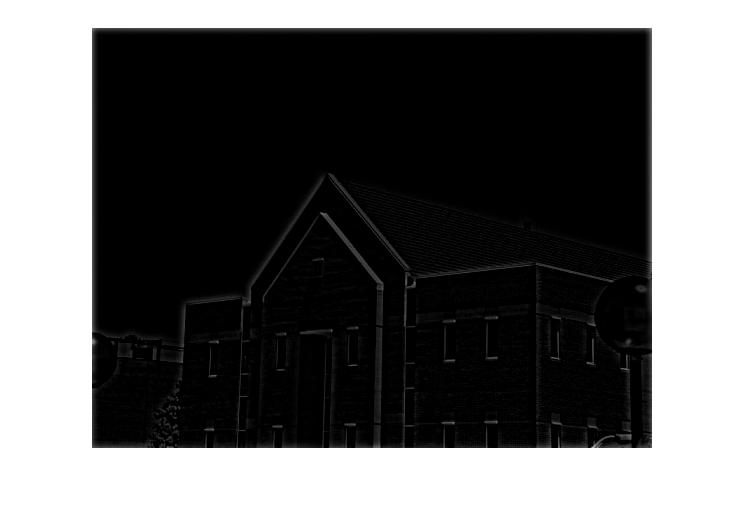
\includegraphics[width=\textwidth]{LoG1.jpg}
		\caption{}
		\label{fig:LoG1}
	\end{subfigure}
	%
	\begin{subfigure}[b]{0.23\textwidth}
		
\includegraphics[width=\textwidth]{LoG2.jpg}
		\caption{}
		\label{fig:LoG2}
	\end{subfigure}
	%
	\begin{subfigure}[b]{0.23\textwidth}
		
\includegraphics[width=\textwidth]{LoG3.jpg}
		\caption{}
		\label{fig:LoG3}
	\end{subfigure}
	%
	\begin{subfigure}[b]{0.23\textwidth}
		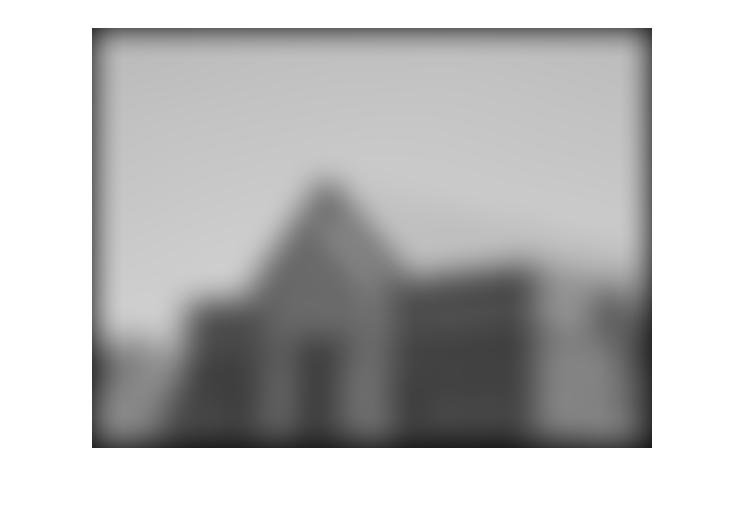
\includegraphics[width=\textwidth]{LoG4.jpg}
		\caption{}
		\label{fig:LoG4}
	\end{subfigure}
	
	\caption{LoG displays per level, from 1 to 4, left to right.}
	\label{fig:LoG}
\end{figure}

\subsection{Part 2b}

The default format for image data in Matlab is \textbf{uint8}. This format does not support negative numbers that result from subtraction of image data matrices (all $L_l[I]$ except for $l=n$), thus when reconstructing back the original image the reconstruction is not accurate (Fig~\ref{fig:rec1b}) and results in a bloom effect. To solve this problem, the image data needs to be converted to \textbf{double}, thus supporting negative values. This allows for an accurate reconstruction (Fig~\ref{fig:rec2b}).

\begin{figure}[!htbp]
	
	\begin{subfigure}[b]{0.48\textwidth}
		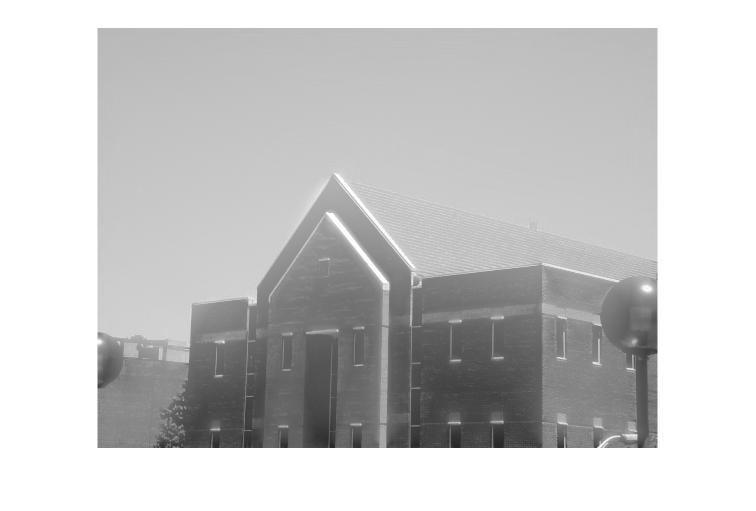
\includegraphics[width=\textwidth]{rec_1_building.jpg}
		\caption{}
		\label{fig:rec1b}
	\end{subfigure}
	%
	\begin{subfigure}[b]{0.48\textwidth}
		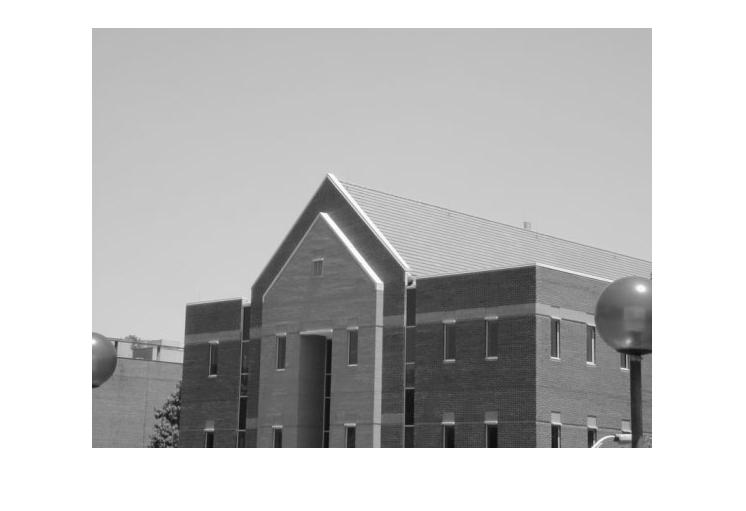
\includegraphics[width=\textwidth]{rec_2_building.jpg}
		\caption{}
		\label{fig:rec2b}
	\end{subfigure}
	
	\caption{\textbf{(a)}: recreated image from uint8 laplacian pyramid. \textbf{(b)}: recreated image from double laplacian pyramid}
	
\end{figure}

\subsection{Part 2c}

Figure \ref{fig:BG_Changed} presents an applied example for the background changing, for a different background than shown in the HW assignment.

\begin{figure}[!htbp]
	\centering
	\begin{subfigure}[b]{0.48\textwidth}
		
		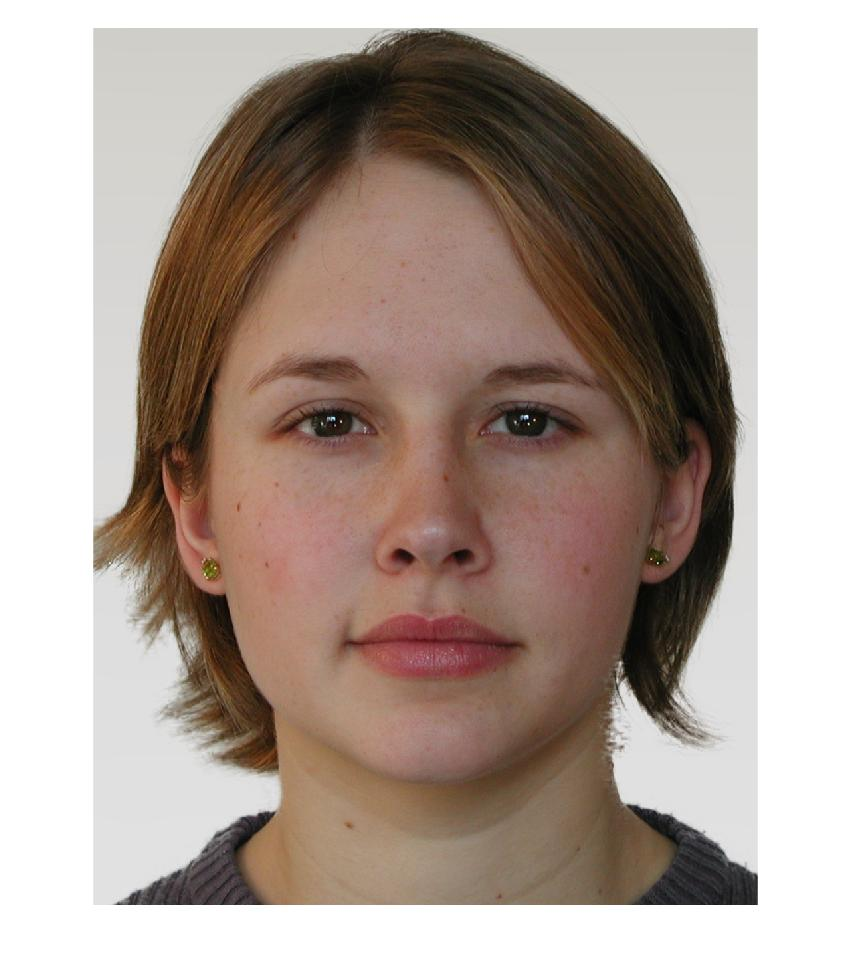
\includegraphics[width=\textwidth]{BG_Changed.jpg}
		
	\end{subfigure}
	\caption{Example image with changed background to image 21.}
	\label{fig:BG_Changed}

\end{figure}

\subsection{Part 2d}

We present a representation of energy of the two example images, input image in Fig.~\ref{fig:150}, style image in Fig.~\ref{fig:100}. These images present successive levels of details, pinpointing with each subsequent level the most important details for both of the images. Black being all channels are 0.

\begin{figure}[!htbp]
	
	\begin{subfigure}[b]{0.15\textwidth}
		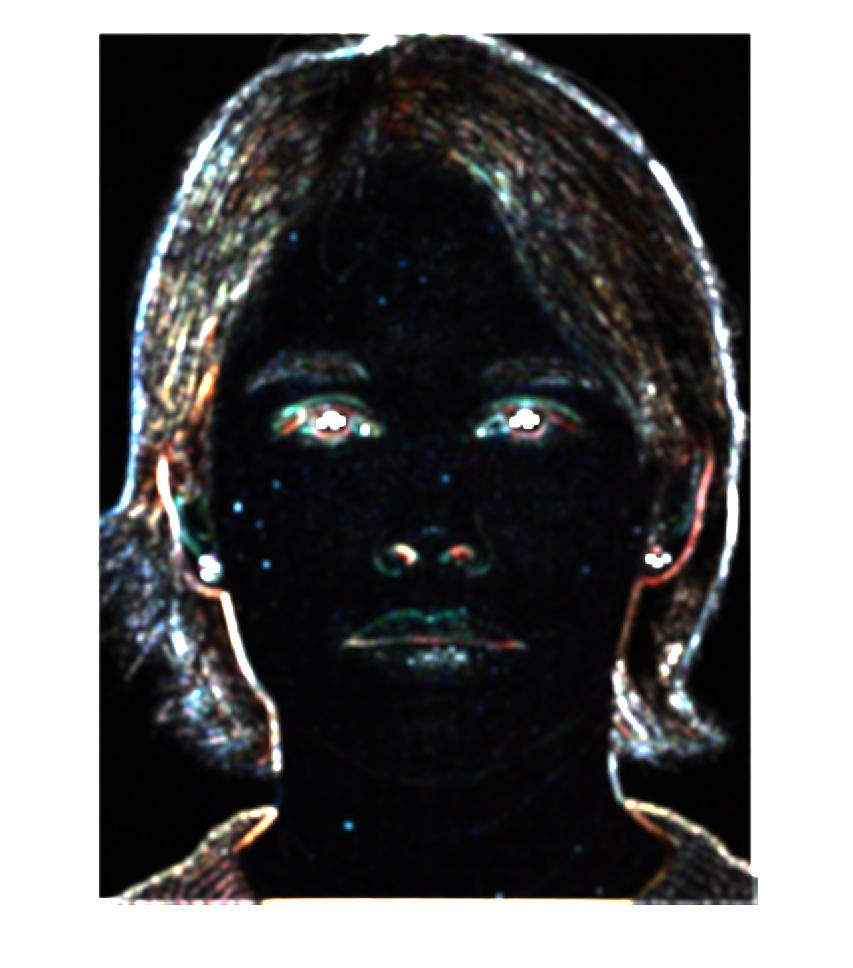
\includegraphics[width=\textwidth]{151.jpg}
		\caption{}
		\label{fig:151}
	\end{subfigure}
	%
	\begin{subfigure}[b]{0.15\textwidth}
		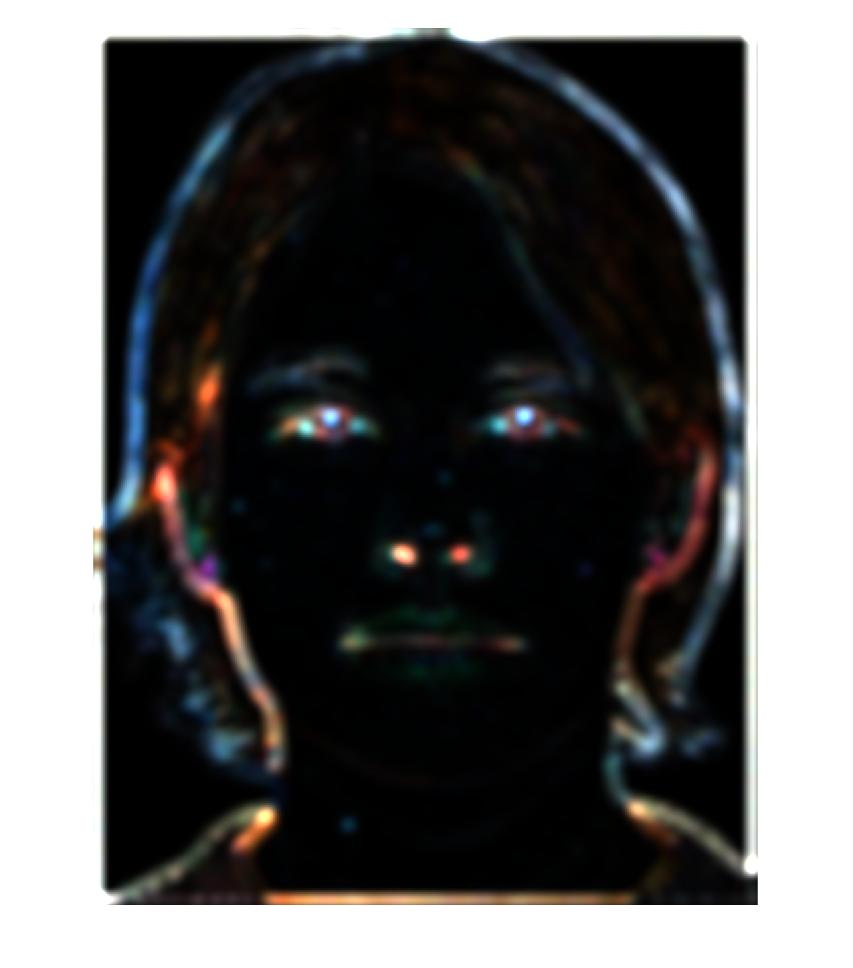
\includegraphics[width=\textwidth]{152.jpg}
		\caption{}
		\label{fig:152}
	\end{subfigure}
	%
	\begin{subfigure}[b]{0.15\textwidth}
		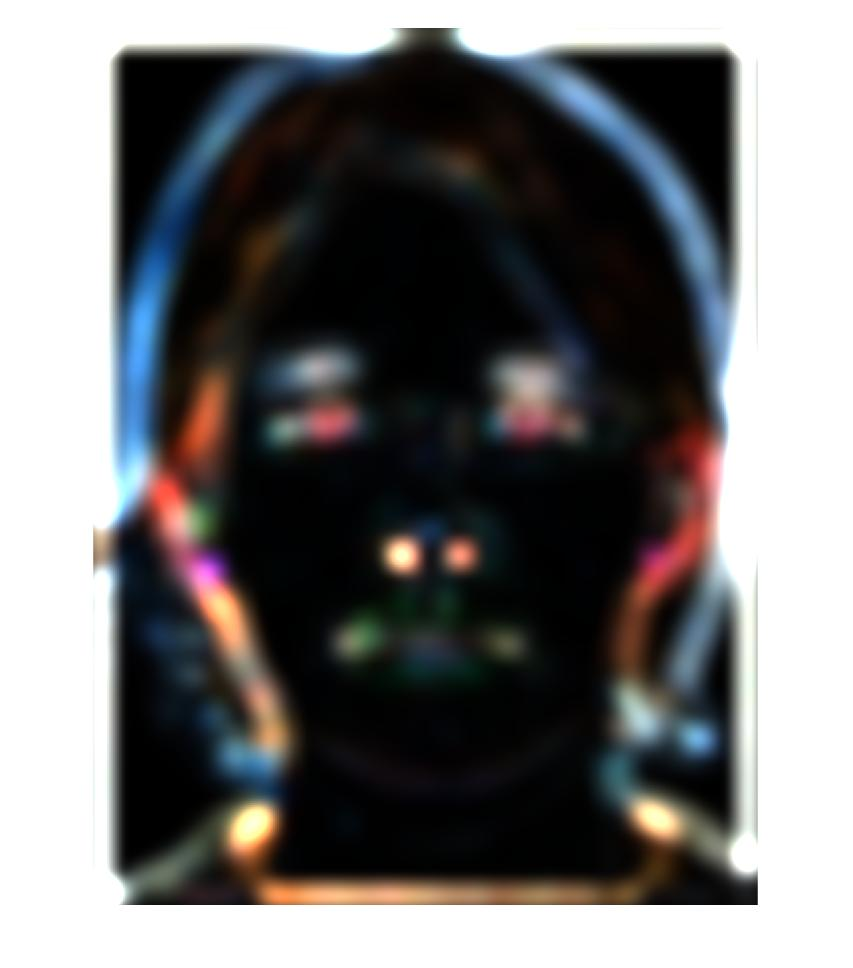
\includegraphics[width=\textwidth]{153.jpg}
		\caption{}
		\label{fig:153}
	\end{subfigure}
	%
	\begin{subfigure}[b]{0.15\textwidth}
		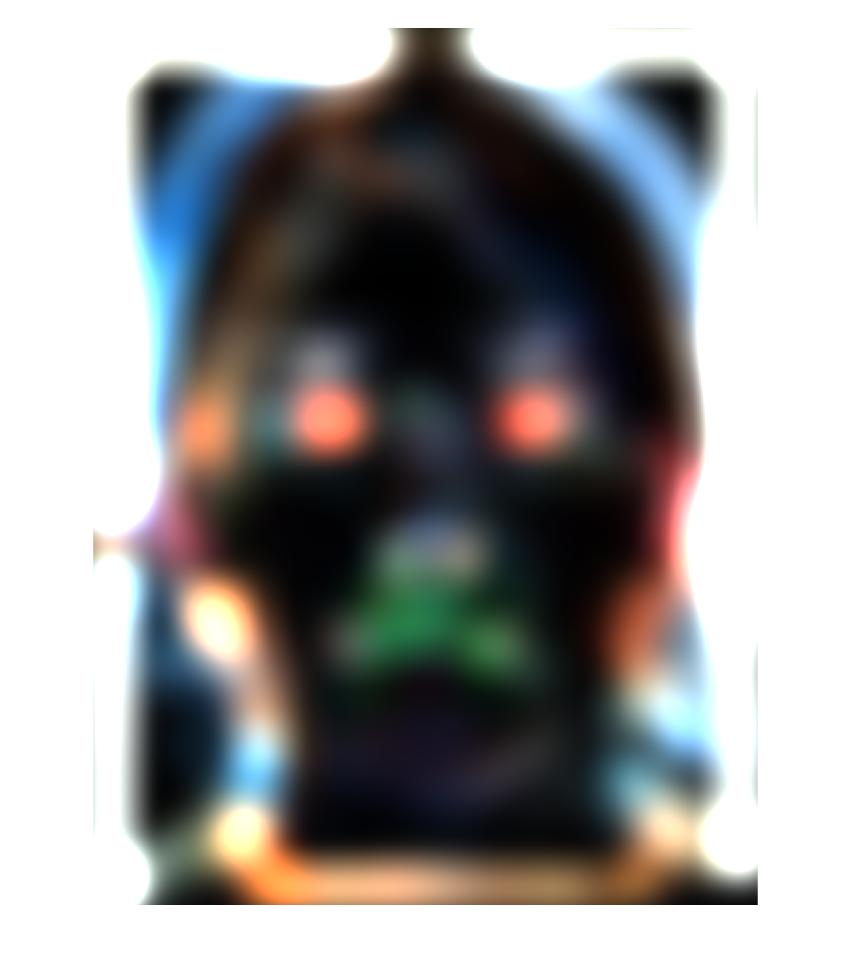
\includegraphics[width=\textwidth]{154.jpg}
		\caption{}
		\label{fig:154}
	\end{subfigure}
	%
	\begin{subfigure}[b]{0.15\textwidth}
		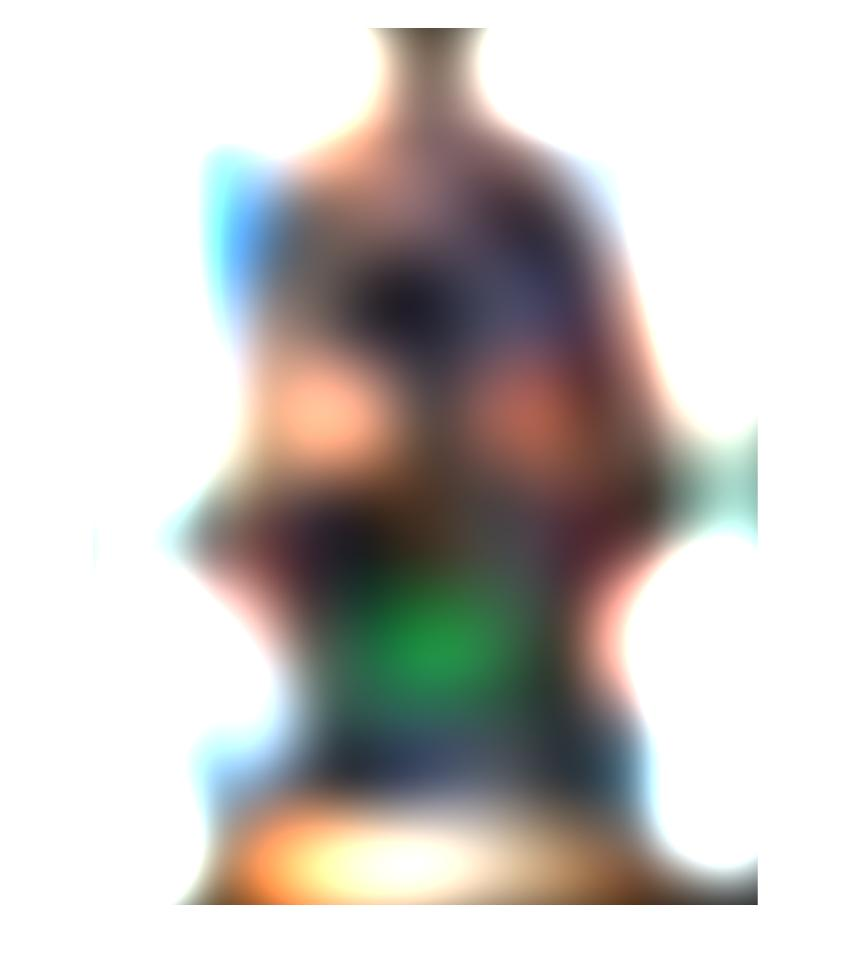
\includegraphics[width=\textwidth]{155.jpg}
		\caption{}
		\label{fig:155}
	\end{subfigure}
	%
	\begin{subfigure}[b]{0.15\textwidth}
		
\includegraphics[width=\textwidth]{156.jpg}
		\caption{}
		\label{fig:156}
	\end{subfigure}
	
	\caption{Energy of input image, from the highest to lowest level, left to right.}
	\label{fig:150}
\end{figure}

\begin{figure}[!htbp]
	
	\begin{subfigure}[b]{0.15\textwidth}
		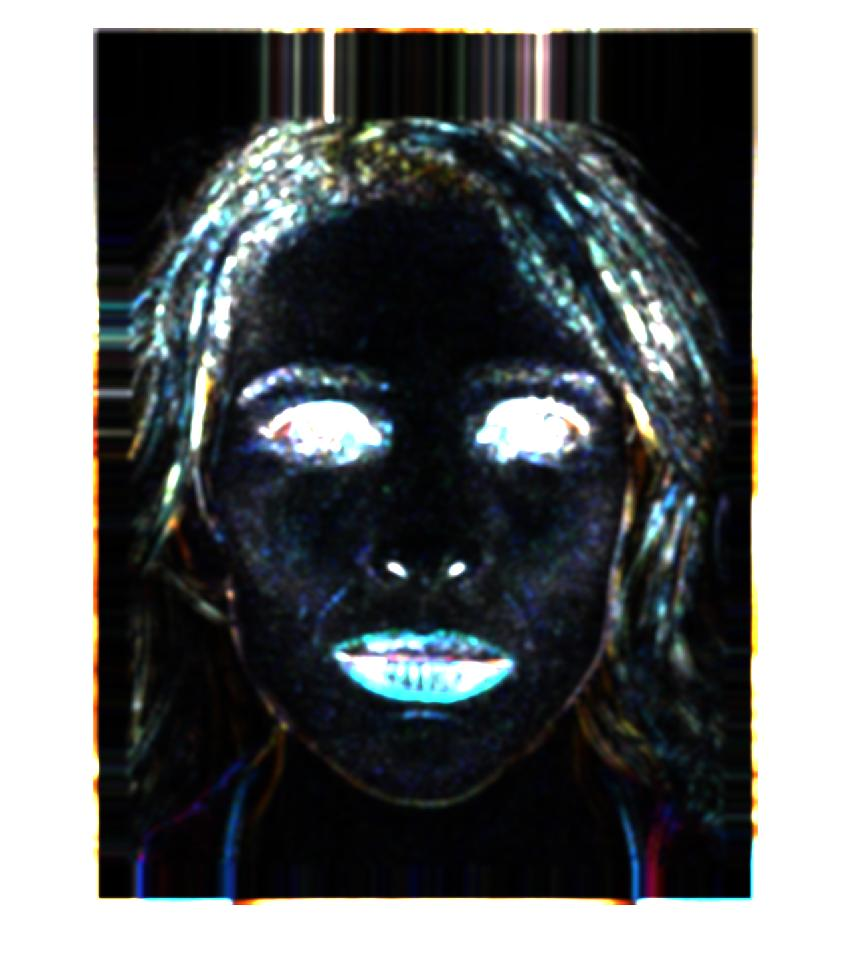
\includegraphics[width=\textwidth]{101.jpg}
		\caption{}
		\label{fig:101}
	\end{subfigure}
	%
	\begin{subfigure}[b]{0.15\textwidth}
		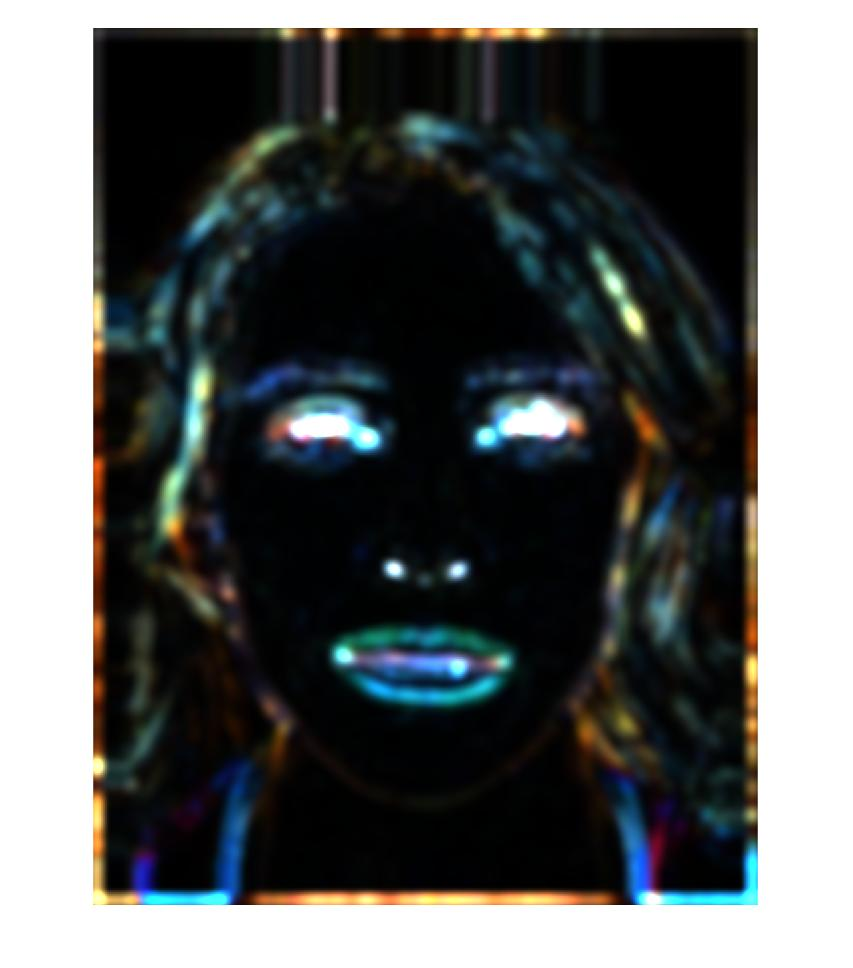
\includegraphics[width=\textwidth]{102.jpg}
		\caption{}
		\label{fig:102}
	\end{subfigure}
	%
	\begin{subfigure}[b]{0.15\textwidth}
		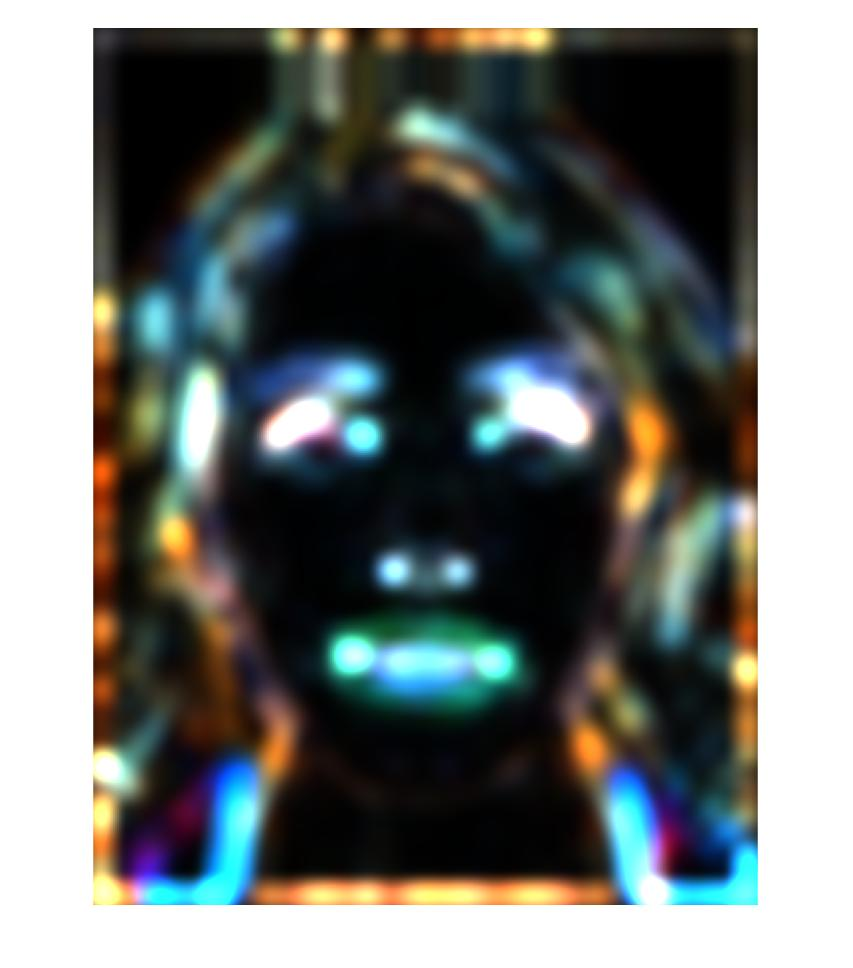
\includegraphics[width=\textwidth]{103.jpg}
		\caption{}
		\label{fig:103}
	\end{subfigure}
	%
	\begin{subfigure}[b]{0.15\textwidth}
		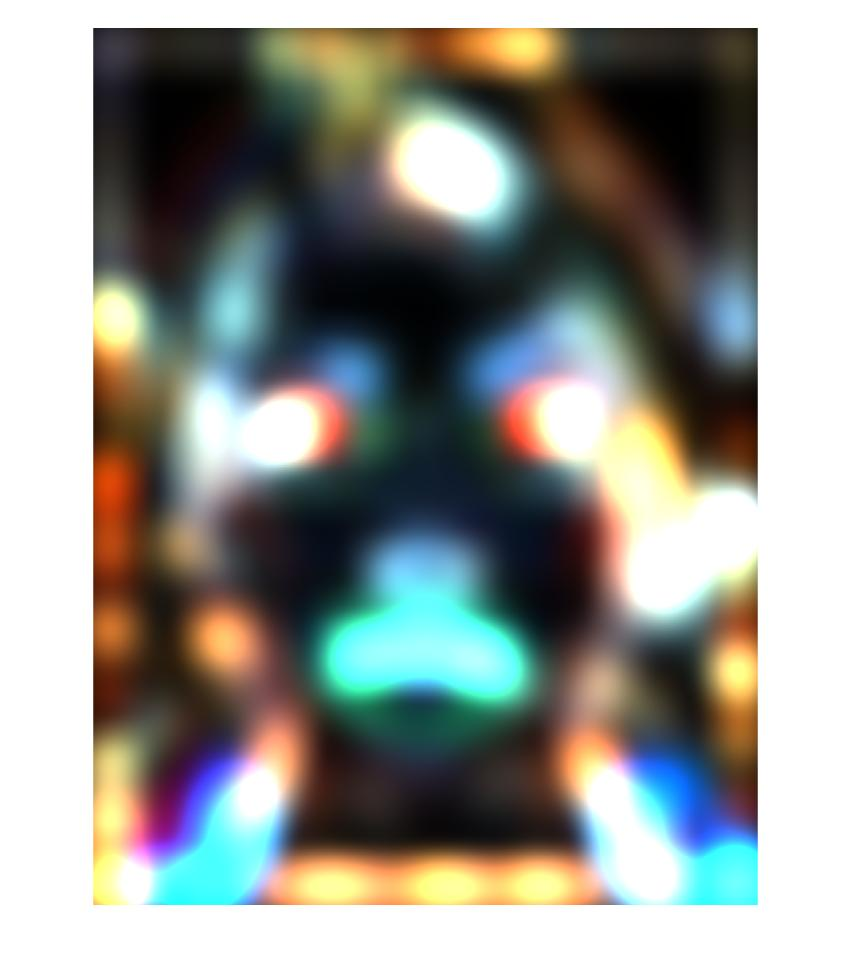
\includegraphics[width=\textwidth]{104.jpg}
		\caption{}
		\label{fig:104}
	\end{subfigure}
	%
	\begin{subfigure}[b]{0.15\textwidth}
		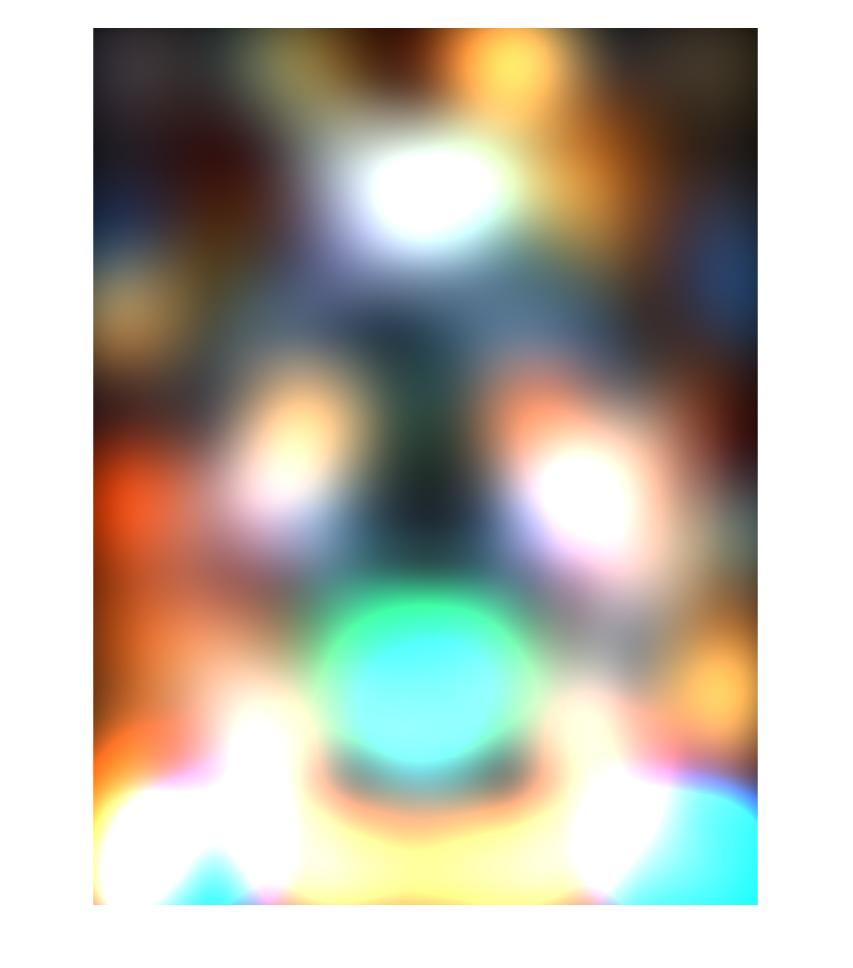
\includegraphics[width=\textwidth]{105.jpg}
		\caption{}
		\label{fig:105}
	\end{subfigure}
	%
	\begin{subfigure}[b]{0.15\textwidth}
		
\includegraphics[width=\textwidth]{106.jpg}
		\caption{}
		\label{fig:106}
	\end{subfigure}
	
	\caption{Energy of style image, from the highest to lowest level, left to right.}
	\label{fig:100}
\end{figure}

Fig.~\ref{fig:200} presents the gain of each pyramid level, presenting the area of influence for each level of the pyramid. For the lower levels, it's evident that the edges are influenced the least. The gain is presented in RGB values, as in uint8 the values are low.

\begin{figure}[!htbp]
	
	\begin{subfigure}[b]{0.15\textwidth}
		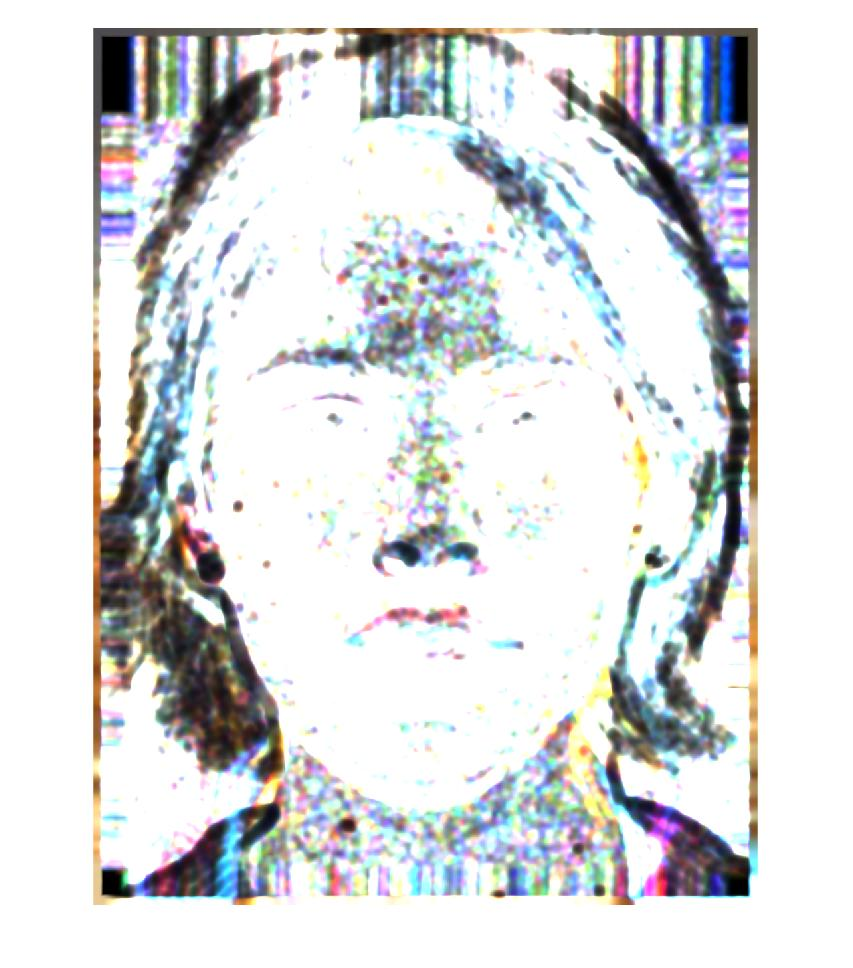
\includegraphics[width=\textwidth]{201.jpg}
		\caption{}
		\label{fig:201}
	\end{subfigure}
	%
	\begin{subfigure}[b]{0.15\textwidth}
		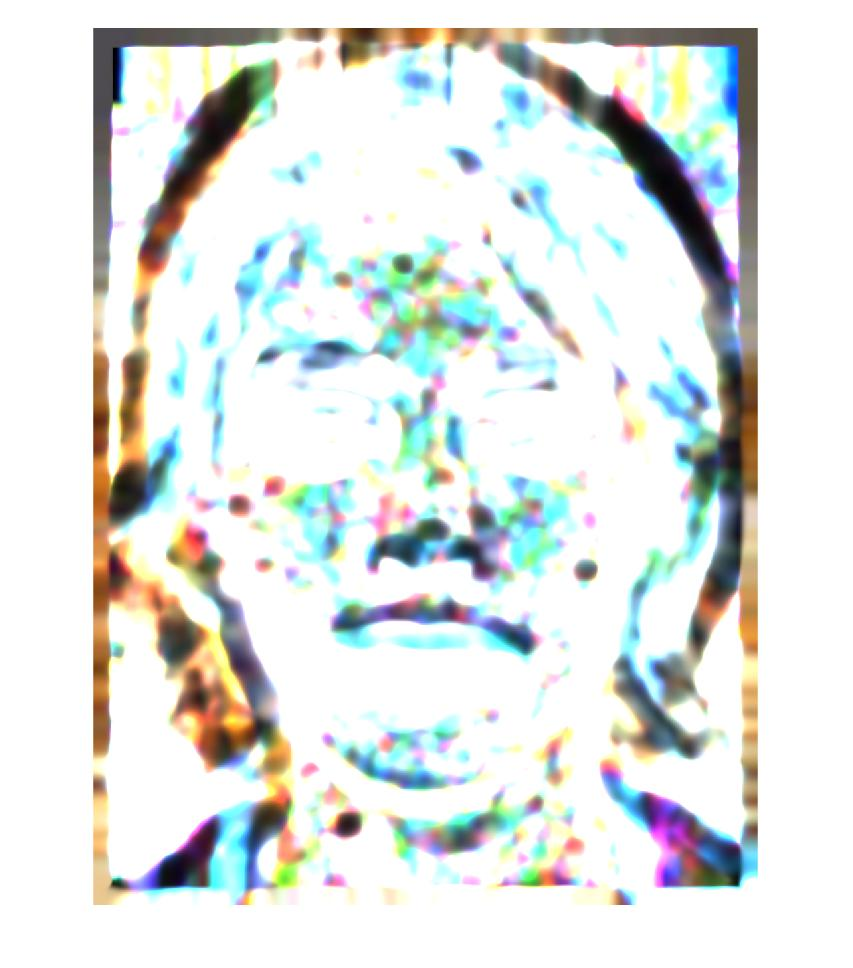
\includegraphics[width=\textwidth]{202.jpg}
		\caption{}
		\label{fig:202}
	\end{subfigure}
	%
	\begin{subfigure}[b]{0.15\textwidth}
		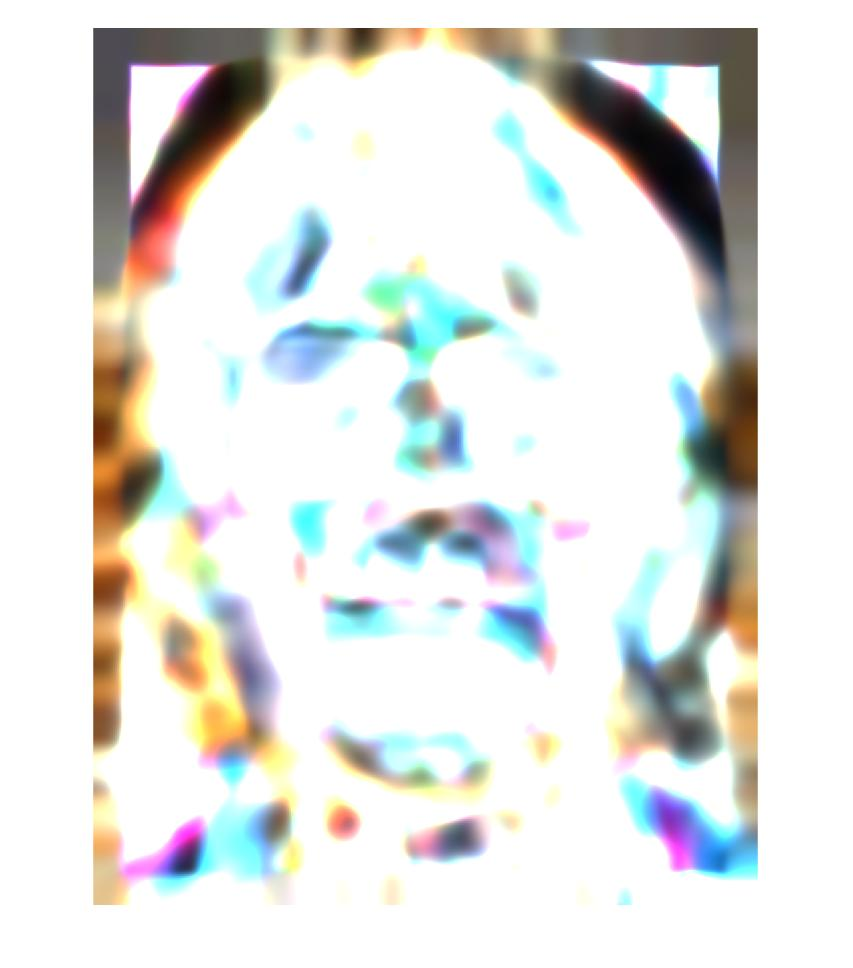
\includegraphics[width=\textwidth]{203.jpg}
		\caption{}
		\label{fig:203}
	\end{subfigure}
	%
	\begin{subfigure}[b]{0.15\textwidth}
		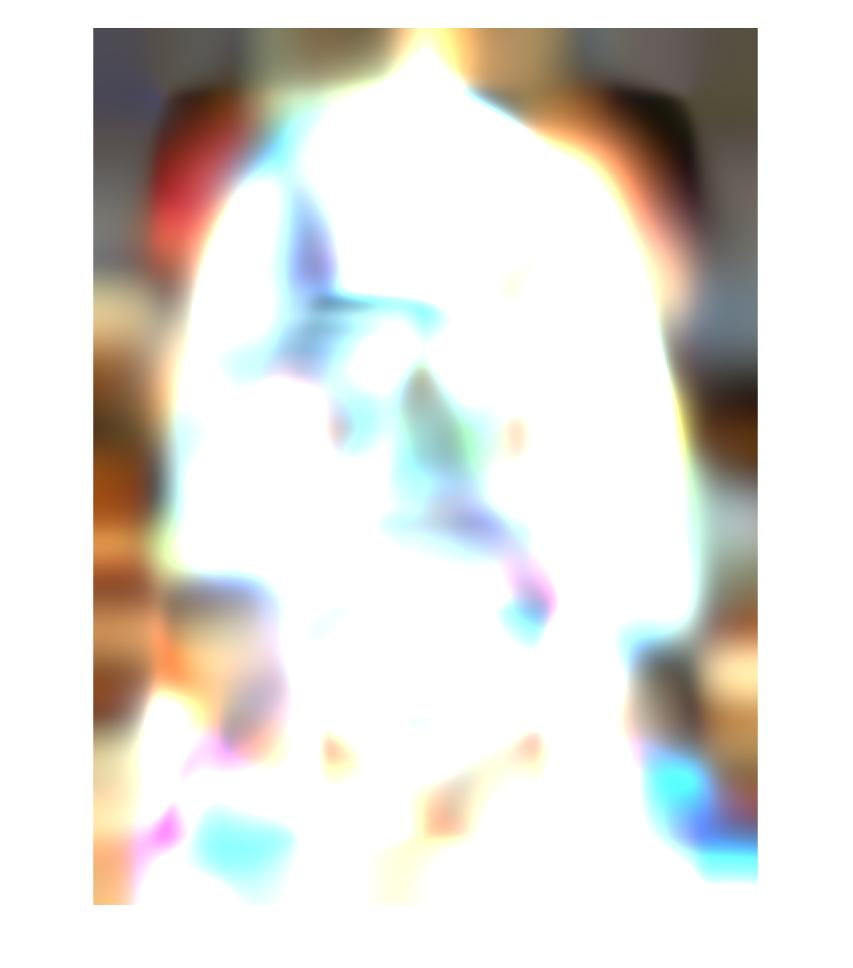
\includegraphics[width=\textwidth]{204.jpg}
		\caption{}
		\label{fig:204}
	\end{subfigure}
	%
	\begin{subfigure}[b]{0.15\textwidth}
		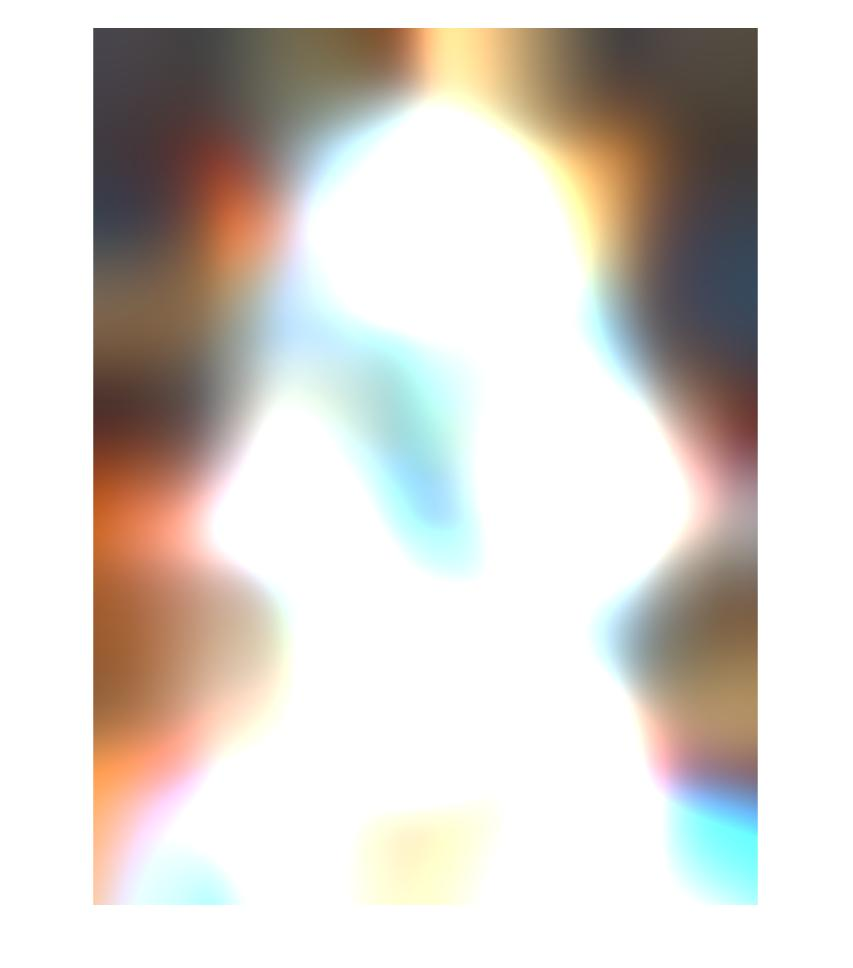
\includegraphics[width=\textwidth]{205.jpg}
		\caption{}
		\label{fig:205}
	\end{subfigure}
	%
	\begin{subfigure}[b]{0.15\textwidth}
		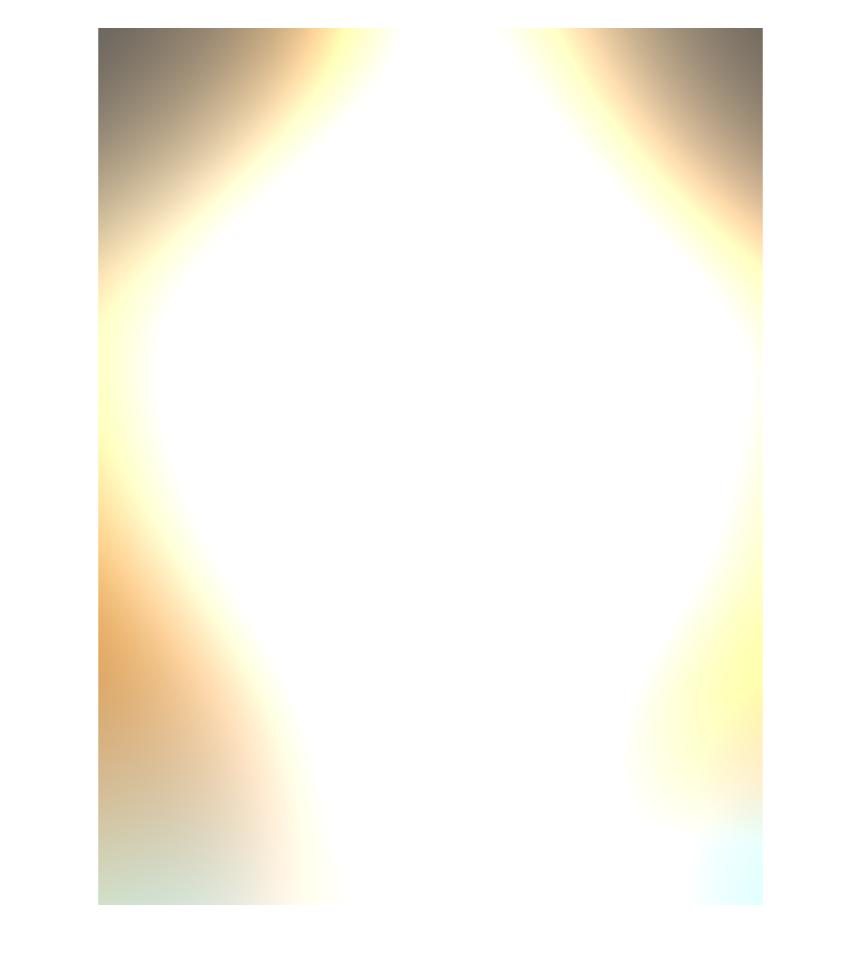
\includegraphics[width=\textwidth]{206.jpg}
		\caption{}
		\label{fig:206}
	\end{subfigure}
	
	\caption{Gain, from the highest to lowest level, left to right.}
	\label{fig:200}
\end{figure}

\subsection{Part 2e}

Output image pyramid is present in Fig.~\ref{fig:400}. It shows a similar pattern presented in Fig.~\ref{fig:LoG}. The edges are representative of the input image, while the highest level presents a blurred version of the style image.

\begin{figure}[!htbp]
	
	\begin{subfigure}[b]{0.15\textwidth}
		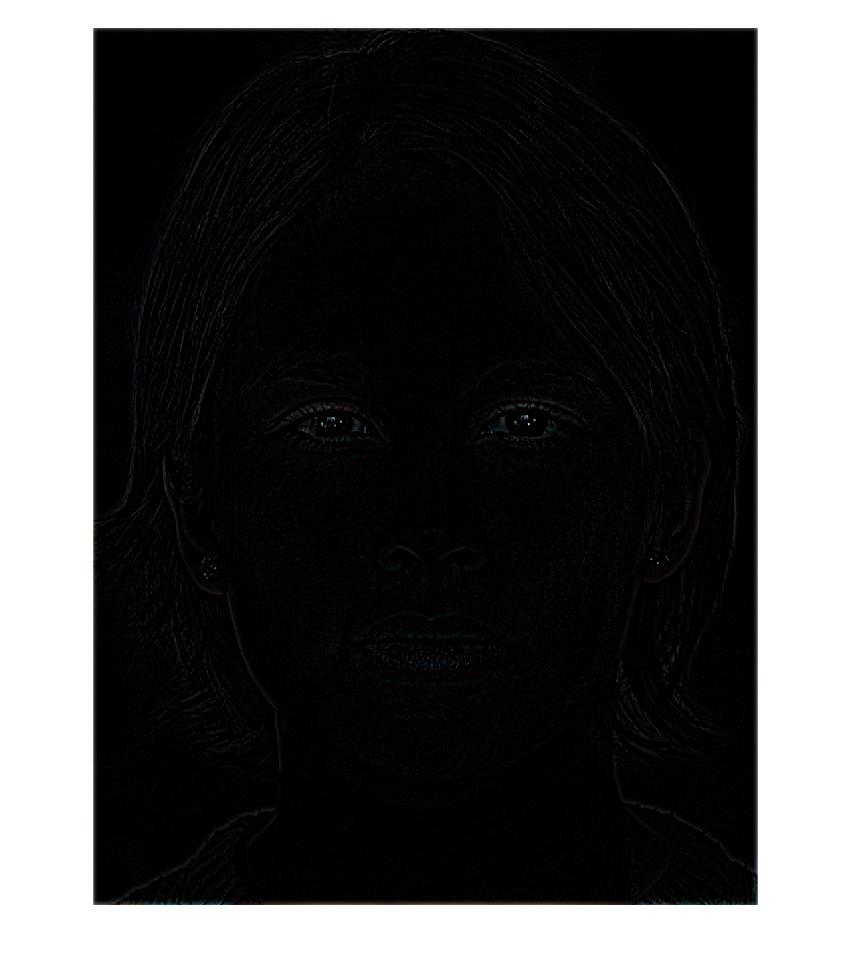
\includegraphics[width=\textwidth]{401.jpg}
		\caption{}
		\label{fig:401}
	\end{subfigure}
	%
	\begin{subfigure}[b]{0.15\textwidth}
		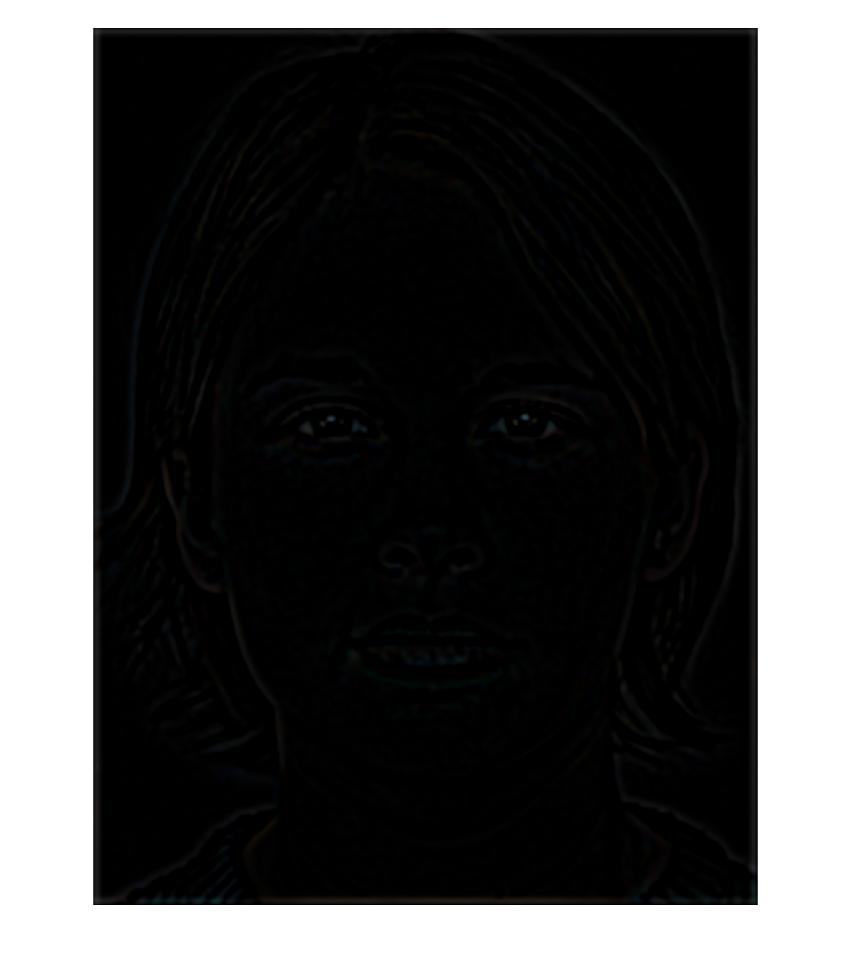
\includegraphics[width=\textwidth]{402.jpg}
		\caption{}
		\label{fig:402}
	\end{subfigure}
	%
	\begin{subfigure}[b]{0.15\textwidth}
		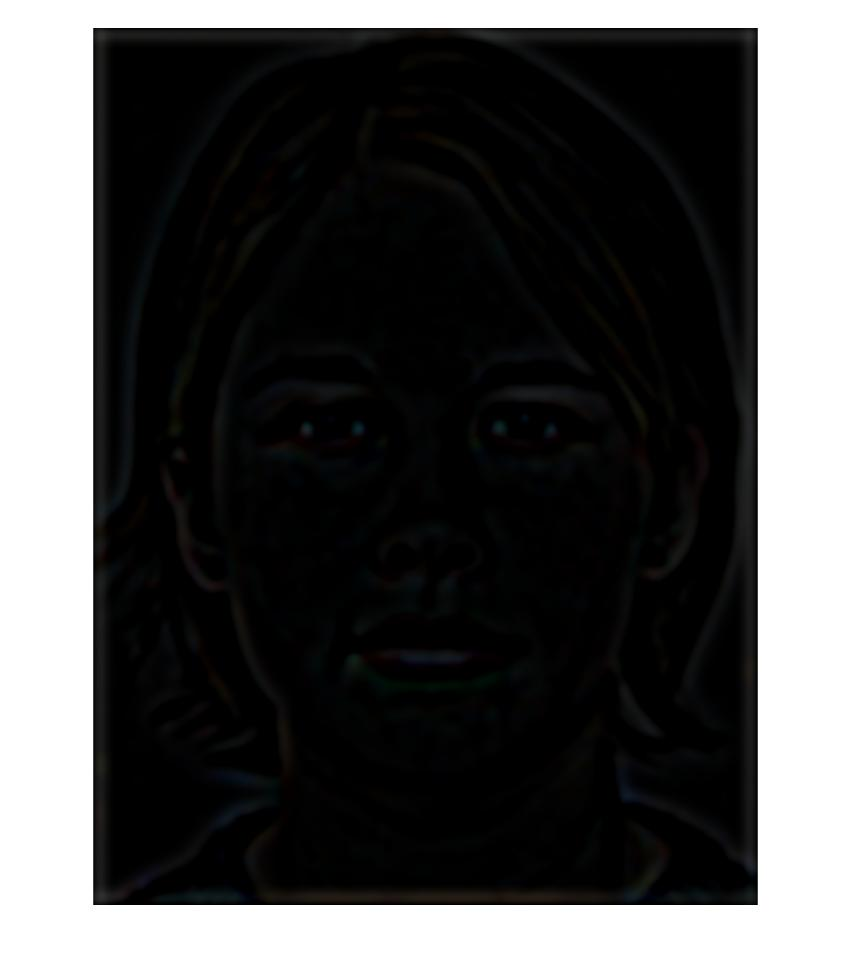
\includegraphics[width=\textwidth]{403.jpg}
		\caption{}
		\label{fig:403}
	\end{subfigure}
	%
	\begin{subfigure}[b]{0.15\textwidth}
		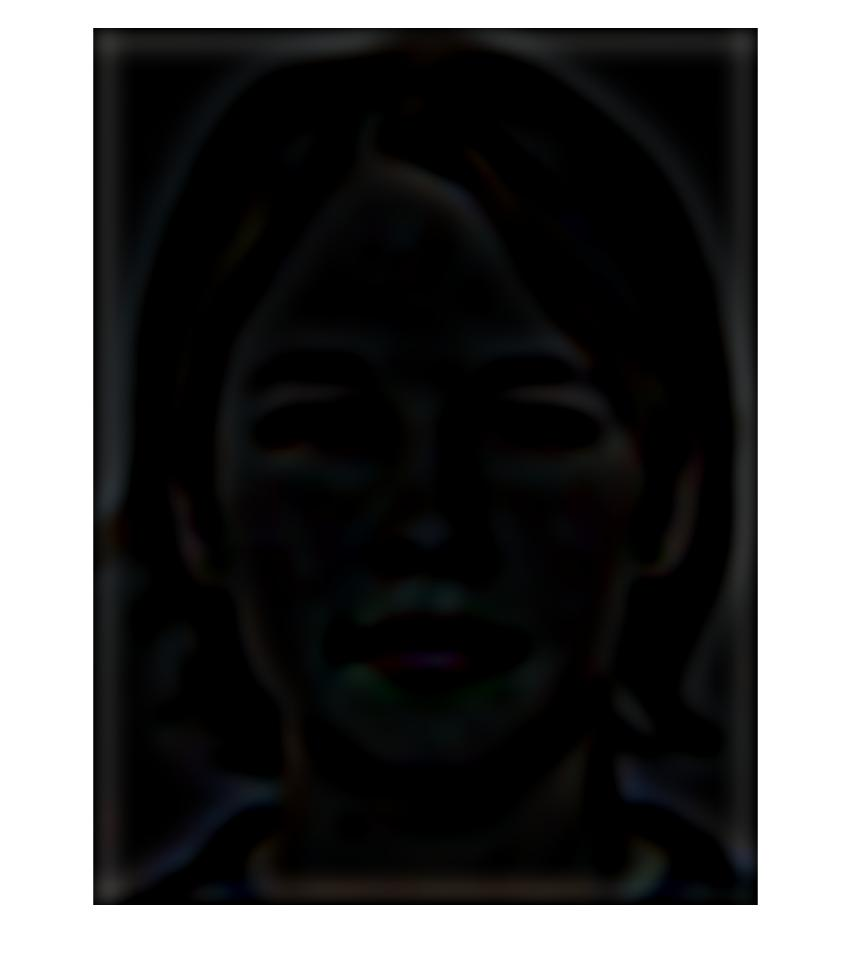
\includegraphics[width=\textwidth]{404.jpg}
		\caption{}
		\label{fig:404}
	\end{subfigure}
	%
	\begin{subfigure}[b]{0.15\textwidth}
		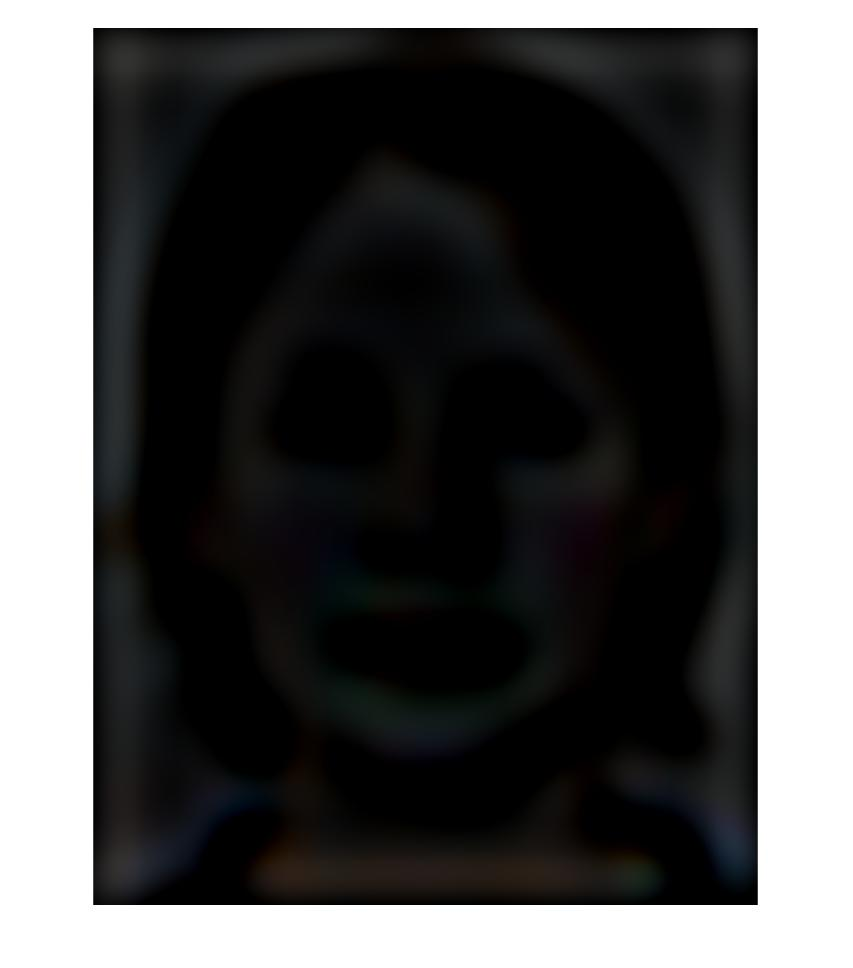
\includegraphics[width=\textwidth]{405.jpg}
		\caption{}
		\label{fig:405}
	\end{subfigure}
	%
	\begin{subfigure}[b]{0.15\textwidth}
		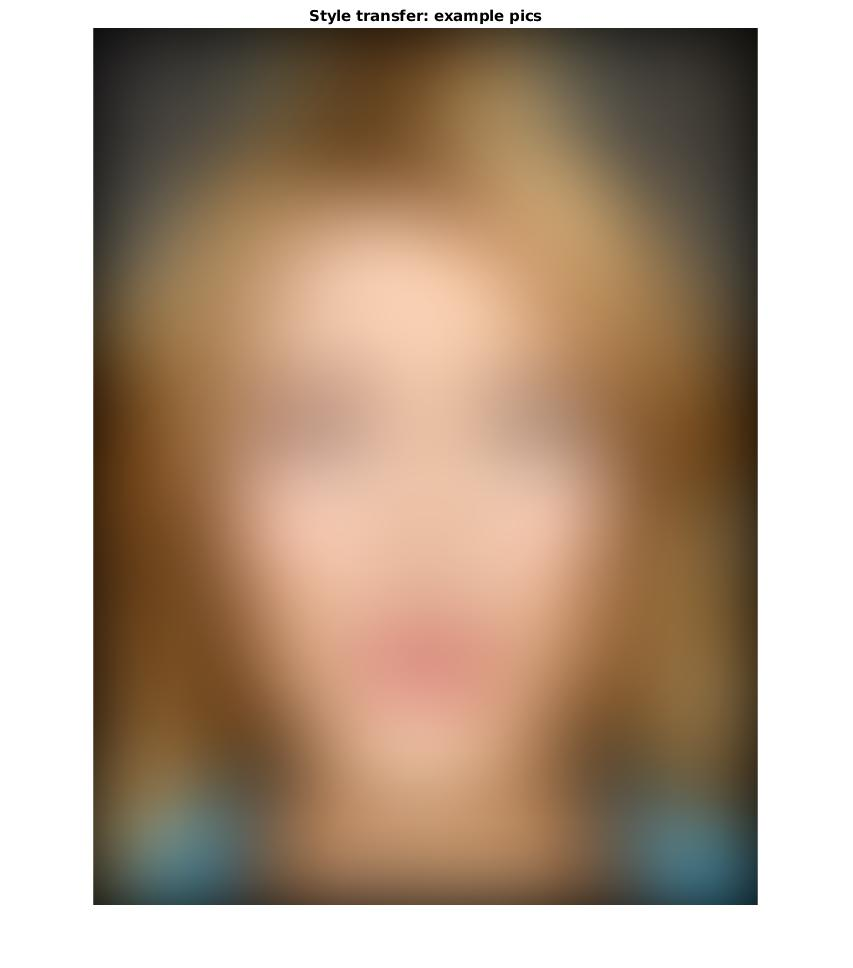
\includegraphics[width=\textwidth]{406.jpg}
		\caption{}
		\label{fig:406}
	\end{subfigure}
	
	\caption{Output image pyramid, from the highest to lowest level, left to right.}
	\label{fig:400}
\end{figure}

\subsection{Part 2f+2g}

In this section we present the style transfer of images of a woman (Fig.~\ref{fig:Woman}, image $0004_6$) and a man (Fig.~\ref{fig:Man}, image $0006_001$) with 3 different styles, one for each image. Note that for image \ref{fig:i_46_21} the style image had a short-haired woman with a light gray background, hence part of the woman's hair is gray. Background in all images is background 21.

\begin{figure}[!htbp]
	
	\begin{subfigure}[b]{0.32\textwidth}
		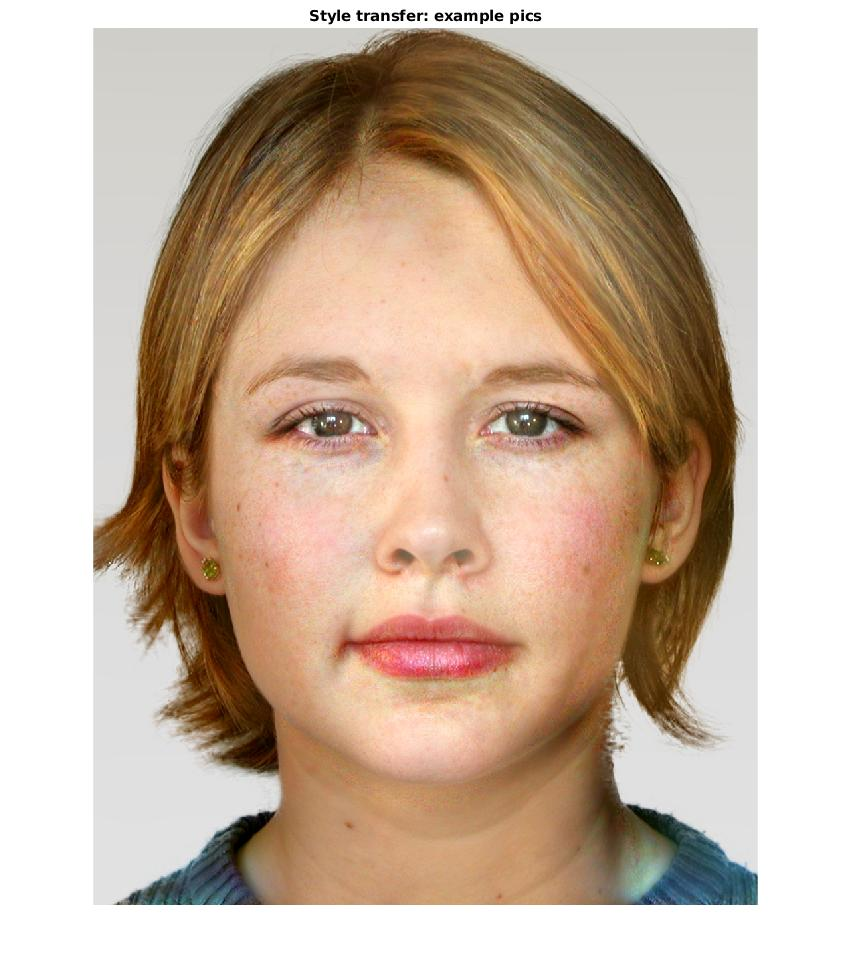
\includegraphics[width=\textwidth]{image_46_6.jpg}
		\caption{}
		\label{fig:i_46_6}
	\end{subfigure}
	%
	\begin{subfigure}[b]{0.32\textwidth}
		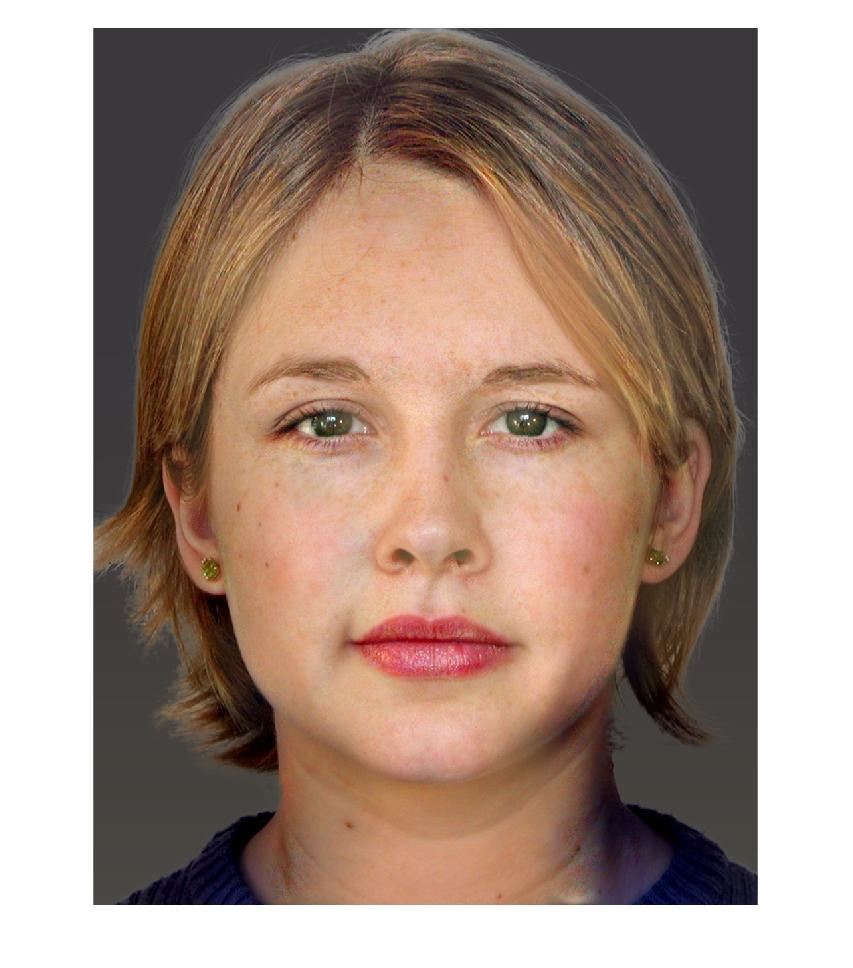
\includegraphics[width=\textwidth]{image_46_16.jpg}
		\caption{}
		\label{fig:i_46_16}
	\end{subfigure}
	%
	\begin{subfigure}[b]{0.32\textwidth}
		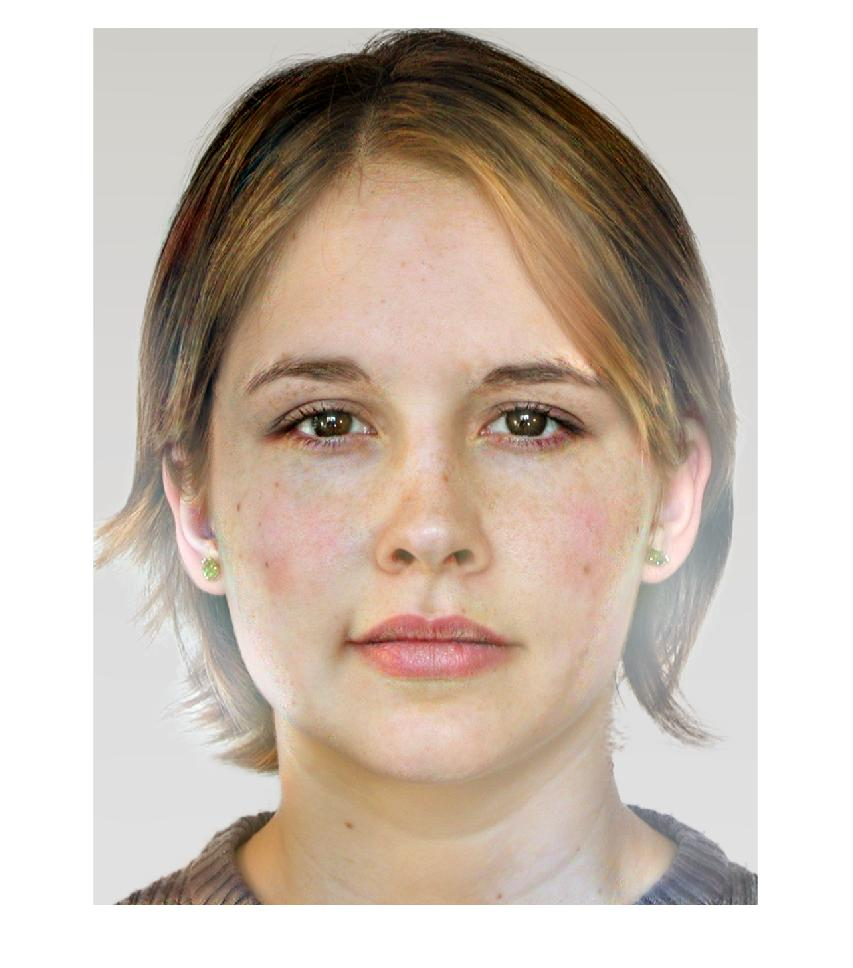
\includegraphics[width=\textwidth]{image_46_21.jpg}
		\caption{}
		\label{fig:i_46_21}
	\end{subfigure}
	
	\caption{Style transfer of the woman photo. \textbf{a} with image 6, \textbf{b} with image 16, \textbf{c} with image 21.}
	\label{fig:Woman}
\end{figure}

\begin{figure}[!htbp]
	
	\begin{subfigure}[b]{0.32\textwidth}
		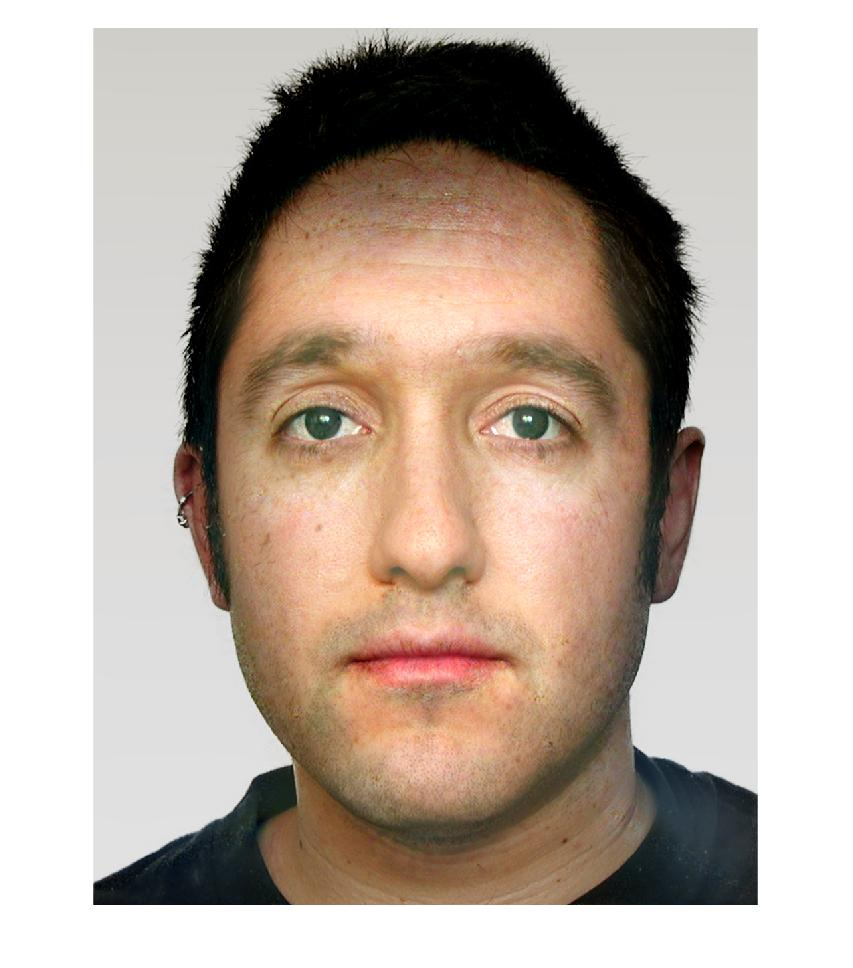
\includegraphics[width=\textwidth]{image_61_0.jpg}
		\caption{}
		\label{fig:i_61_0}
	\end{subfigure}
	%
	\begin{subfigure}[b]{0.32\textwidth}
		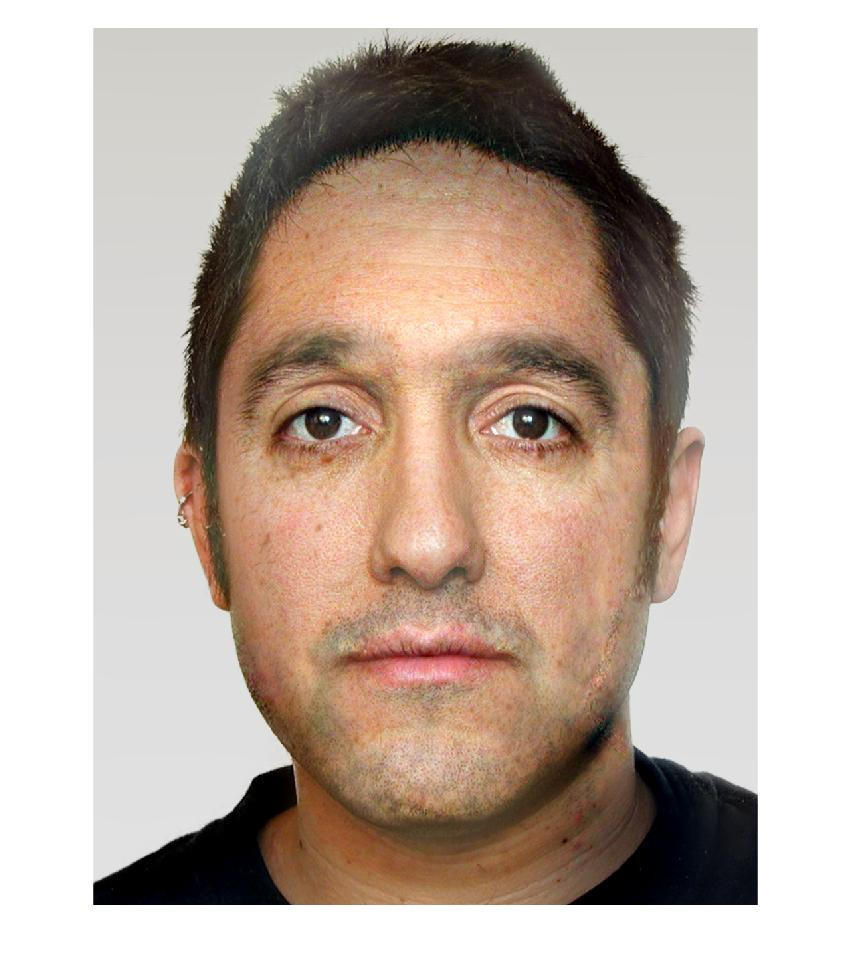
\includegraphics[width=\textwidth]{image_61_9.jpg}
		\caption{}
		\label{fig:i_61_9}
	\end{subfigure}
	%
	\begin{subfigure}[b]{0.32\textwidth}
		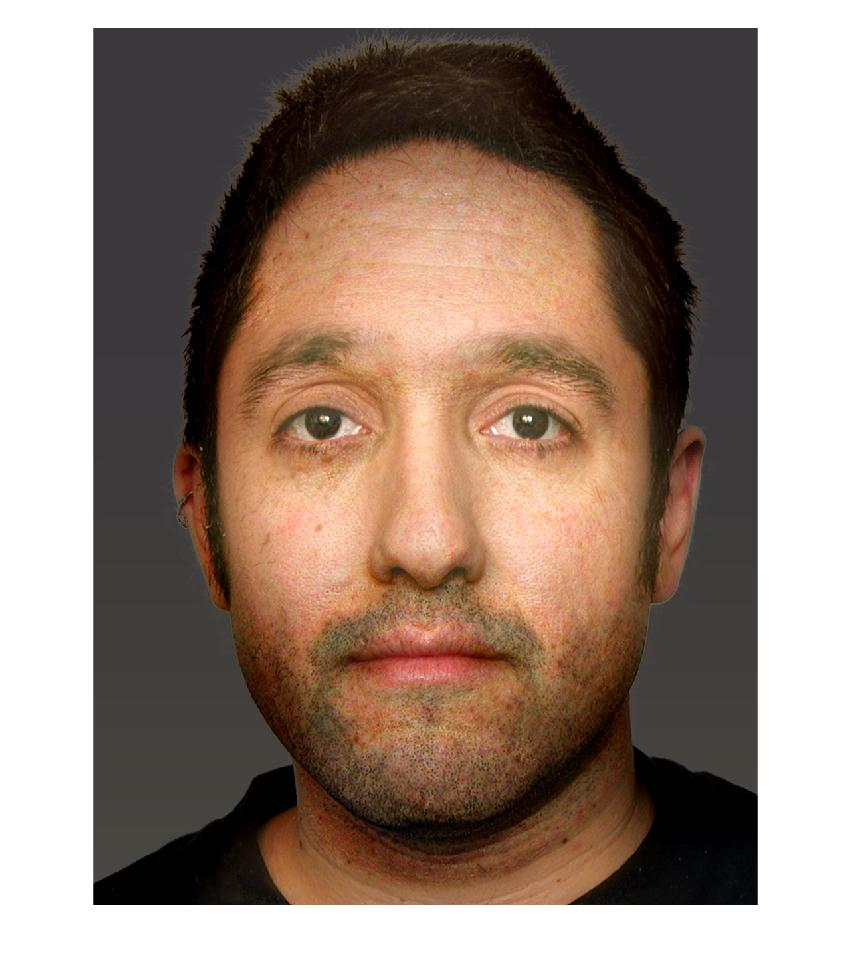
\includegraphics[width=\textwidth]{image_61_10.jpg}
		\caption{}
		\label{fig:i_61_10}
	\end{subfigure}
	
	\caption{Style transfer of the man photo. \textbf{a} with image 0, \textbf{b} with image 9, \textbf{c} with image 10.}
	\label{fig:Man}
\end{figure}

\subsection{Part 2h}

In Fig.~\ref{fig:Custom} we present a style transfer for a painting made by one of the submitters to Van Gogh's Starry Night. The result is presented in Fig.~\ref{fig:image_fused_custom}; the style transfer changed the color scheme and some of the textures. Note that in Starry Night the top right yellow circle is transfered profoundly to the style transfer image.

\begin{figure}[!htbp]
	
	\begin{subfigure}[b]{0.48\textwidth}
		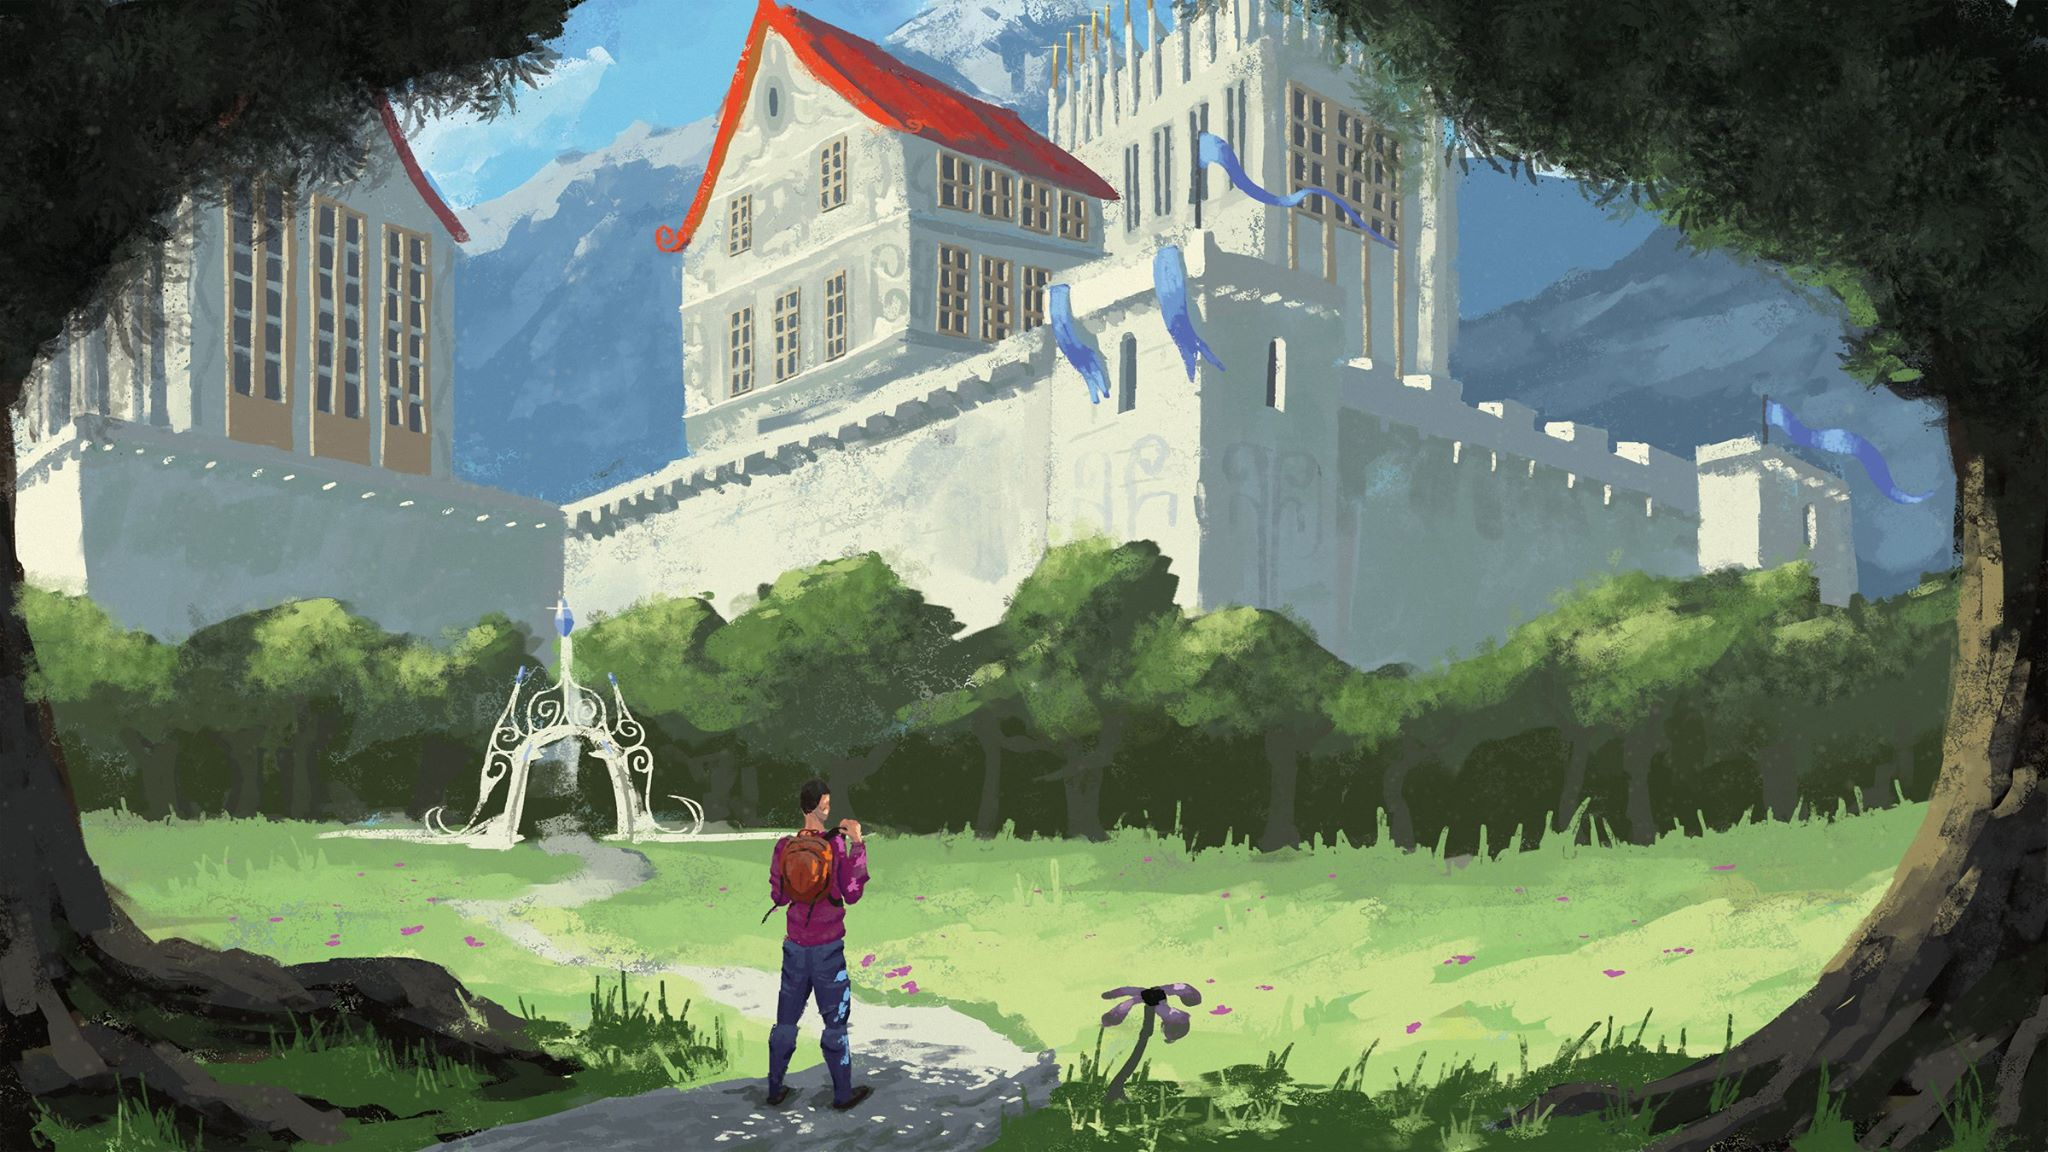
\includegraphics[width=\textwidth]{my_pic.jpg}
		\caption{}
		\label{fig:image_1_custom}
	\end{subfigure}
	%
	\begin{subfigure}[b]{0.48\textwidth}
		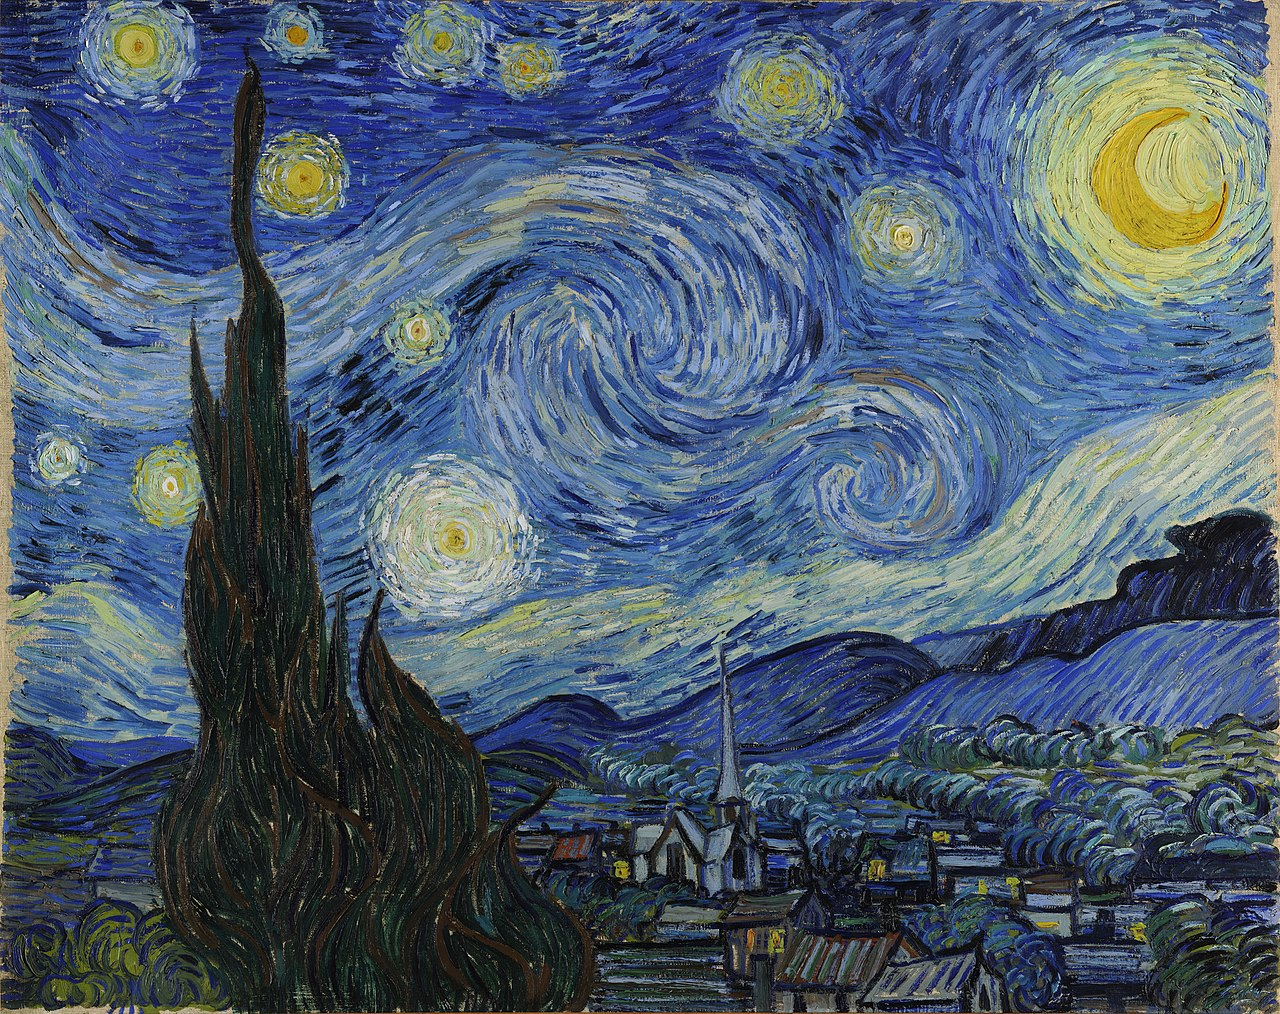
\includegraphics[width=\textwidth]{starry_night.jpg}
		\caption{}
		\label{fig:image_2_custom}
	\end{subfigure}

	\begin{subfigure}[b]{0.65\textwidth}
		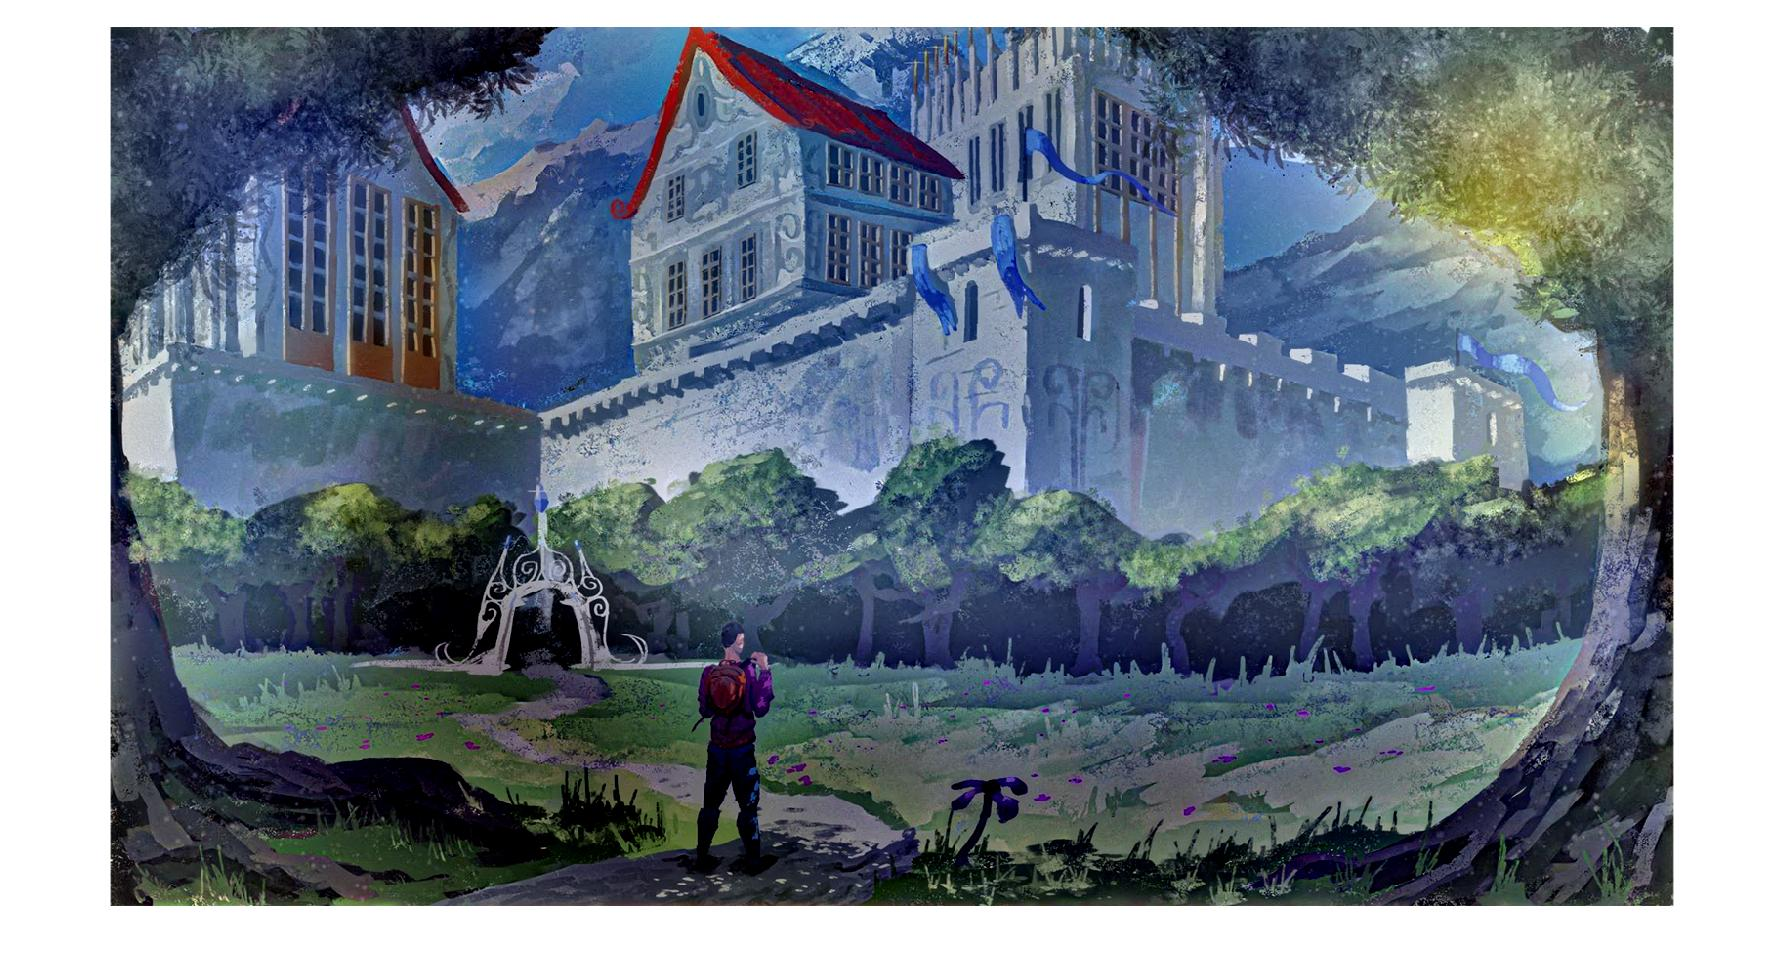
\includegraphics[width=\textwidth]{image_custom.jpg}
		\caption{}
		\label{fig:image_fused_custom}
	\end{subfigure}
	
	\caption{\textbf{a} a painting destined to style transfer. \textbf{b} Starry Night by Van Gogh. \textbf{c} the style transfered painting.}
	\label{fig:Custom}
\end{figure}

\end{document}




